\documentclass[12pt,oneside]{memoir}

\usepackage[biblatex]{matfmaster}
\usepackage{listings}
\usepackage{longtable}

\makeatletter
\def\nobreakhline{%
  \noalign{\ifnum0=`}\fi
    \penalty\@M
    \futurelet\@let@token\LT@@nobreakhline}
\def\LT@@nobreakhline{%
  \ifx\@let@token\hline
    \global\let\@gtempa\@gobble
    \gdef\LT@sep{\penalty\@M\vskip\doublerulesep}% <-- change here
  \else
    \global\let\@gtempa\@empty
    \gdef\LT@sep{\penalty\@M\vskip-\arrayrulewidth}% <-- change here
  \fi
  \ifnum0=`{\fi}%
  \multispan\LT@cols
     \unskip\leaders\hrule\@height\arrayrulewidth\hfill\cr
  \noalign{\LT@sep}%
  \multispan\LT@cols
     \unskip\leaders\hrule\@height\arrayrulewidth\hfill\cr
  \noalign{\penalty\@M}%
  \@gtempa}
\makeatother

\bib{master}

\autor{Милош Самарџија}
\naslov{Развој микросервисне апликације за Android коришћењем окружења Lumen}
\godina{2021}

\mentor{др Милена \textsc{Вујошевић Јаничић}, ванредни професор\\ Универзитет у Београду, Математички факултет}
\komisijaA{др Филип \textsc{Марић}, ванредни професор\\ Универзитет у Београду, Математички факултет}
\komisijaB{др Александар \textsc{Картељ}, доцент\\ Универзитет у Београду, Математички факултет}

% \datumodbrane{ }

\apstr{Микросервисна архитектура представљa популаран приступ развоју скалабилних дистрибуираних система са сложеним доменом. Овако добијени системи су лако прошириви и једноставнији су за одржавање. Циљ овог рада је да обради битне концепте микросервисне архитектуре, као и филозофију на којој је ова архитектура заснована. Развијена је апликација која представља конкретан пример микросервисне архитектуре у пракси, дате су препоруке за тестирање и пуштање оваквих система у рад и приказане су предности и мане оваквог приступа развоју софтвера.}

\kljucnereci{дистрибуирано програмирање, доменски оријентисано моделовање, микросервисна архитектура, Docker, Lumen, Android, трчање}

\begin{document}

\frontmatter
\naslovna
\komisija
\posveta{Мојој породици и пријатељима за безусловну подршку}
\apstrakt
\tableofcontents*

\mainmatter

\chapter{Увод}
Микросервисна архитектура представљa популаран приступ развоју скалабилних дистрибуираних система. Главна филозофија на којој је овај приступ заснован је доменски оријентисано моделовање (енг.~\textit{domain-driven design}), које подстиче разбијање сложених домена на што једноставније и независније поддомене.

Главна тематика којом се овај рад бави су основне идеје водиље доменски оријентисаног моделовања, начин на који их микросервисна архитектура уграђује, као и дизајн REST (енг.~\textit{representational state transfer}) интерфејса за програмирање апликација (енг.~\textit{RESTful API}) који представљa једну од техника за интеграцију поддомена система. У те сврхе је осмишљенa и развијена апликација чији је циљ да илуструје примену микросервисне архитектуре у пракси, као и комуникацију са спољним сервисима.

Апликација је названа \textit{My Running Buddy}, а њена примарна намена је проналажење партнера за трчање на основу различитих параметара. Сам алгоритам за упаривање тркача уједно представљa и најважнији поддомен (енг.~\textit{core subdomain}) целог система, и на њега је потребно обратити највише пажњe током дизајна и имплементације. Део апликације је написан у програмском језику PHP коришћењем Lumen развојног оквира за развој микросервисних апликација и REST интерфејса за програмирање апликација, где је највећи део доменске логике садржан. Други део апликације је написан у програмском језику Јава, заједно са Android комплетом за развој софтвера (енг.~\textit{Android SDK}) и представља кориснички интерфејс, односно улазну тачку у систем. За потребе складиштењa података од стране микросервиса користи се систем за управљање базама података MySQL.

У поглављу \ref{domenskiorijentisanomodelovanje} се обрађује доменски оријентисано моделовање, односно, основни концепти, циљеви и препоруке филозофије. Ово поглавље је кључно за разумевање сврхе микросервиса, на који начин се систем разбија на сервисе и колика грануларност тих сервиса треба да буде. Микросервисна архитектура није први и једини архитектурални стил који је увео поделу система на сервисе; без разумевања идеологије коју заступа, тешко би било уочити разлику између микросервиса и било које друге сличне архитектуре. Поглавље \ref{mikroservisi} успоставља везу између микросервиса и доменски оријентисаног моделовања, анализира најважније предности и мане оваквог дизајна, и обрађује теме везане за упошљавање микросервиса и њихово тестирање. Поглавље \ref{prakticnideo} укратко даје преглед технологија употребљених у пројекту, описује процес креирања апликације, од фазе планирања и дизајна, па све до најбитнијих имплементационих детаља и изазова. На крају, у последњем поглављу, изведен је закључак где су сумирани доприноси, и утисци стечени током израде рада.

\chapter{Доменски оријентисано моделовање}\label{domenskiorijentisanomodelovanje}
Доменски оријентисано моделовање је филозофија развоја чији циљ је управљање конструкцијом и одржавањем софтвера писаног за сложене домене \cite{DomainDrivenDessign}. Циљ се достиже употребом одређених образаца (енг.~\textit{patterns}), принципа и добрих пракси које, уколико се добро разумеју и примене, смањују шансу за прављење неких честих грешака које се јављају током развоја.

\section{Идеја филозофије и основни концепти}
Идеја водиља ове филозофије је разбијање великих и сложених домена на једноставније поддомене. Ово има двојаки значај:
\begin{enumerate}
\item добијамо поддомене који су мање сложени, и који имају јаснију одговорност;
\item лакше се проналазе и изолују најважнији поддомени у које је потребно уложити највећи део времена, јер је то оно што одређени софтвер чини другачијим од осталих решења, и представља разлог због којег је уопште и настао.
\end{enumerate}

Такође, филозофија инсистира на томе да се у пројекат активно укључе и доменски експерти (енг.~\textit{domain experts}) чија би примарна улога била упознавање програмера и остатка тима са сложеним доменом како би се избегле недоумице и погрешна решења. Ово функционише тако што се током целог развојног циклуса организују формални и неформални састанци са експертима, где се кроз дискусију и различите активности (енг.~\textit{knowledge crunching}) врши анализа и разбијање домена на више мањих, и моделовање поддомена. Као резултат ових састанака настају аналитички модел, и заједнички језик (енг.~\textit{ubiquitous language}) чија је улога избегавање двосмислености у комуникацији између експерата и програмера. Током животног циклуса пројекта разумевање домена постаје боље, а заједно са разумевањем се развијају и расту заједнички језик и модели. Сва комуникација, модели и кôд су изражени у терминима заједничког језика.

\subsection{Чести проблеми развоја сложених апликација}
Да бисмо разумели сврху постојања ове филозофије, потребно је да разумемо на какве изазове се најчешће наилази током развоја и одржавања софтвера. Један од популарнијих архитектуралних стилова коришћених у сложеним апликацијама је тзв. "велика лопта од блата" (енг.~\textit{Big Ball of Mud}) коју карактерише лош дизајн кода са одсуством било какве организације. Такав софтвер је углавном доста спрегнут, и захтев за променом једне од функционалности може изазвати ланчану реакцију других измена које нису планиране, али су у том случају неопходне. Проблем је то што није лако уочљиво када пројекат скрене са правог пута, и од добре архитектуре дође до "велике лопте од блата". Временом се софтвер инкрементално квари, додавањем нових функционалности, и "крпљењем" постојећих, уз слабу бригу о одржању архитектуре, са изговором да ће некад касније бити издвојено време за рефакторисање. Тако настаје технички дуг (енг.~\textit{technical debt}).

Технички дуг је концепт у развоју софтвера настао као еквивалент новчаног дуга. Суштина концепта је да, занемаривањем дизајна кода, дуг постаје све већи, и све је мање вероватно да ће бити успешно измирен. У преводу, долази се до стадијума када је свака измена спецификације (која даље повлачи измене у коду) болна јер је софтвер постао изузетно спрегнут, и много компоненти зависи од других, иако у природи можда чак и не постоји таква веза између тих ентитета. Немогуће је направити изоловане измене, већ су оне раштркане широм система, и због тога се веома лако могу увести нове грешке (енг.~\textit{bugs}) у систем.

Јасно је да су измене спецификације неизбежне, па нам једино преостаје да се прилагодимо; у супротном, велика је вероватноћа да ће пројекат бити неуспешан, делимично функционалан и/или тежак за одржавање. У тој ситуацији се, у зависности од тренутног стања кода, долази до закључка да је неопходно извршити опширно рефакторисање, или дизајнирање и писање софтвера испочетка. То све доводи до већих трошкова развоја, који су се могли избећи.

\subsection{Аналитички модел}
Аналитички модел је колекција артефаката који описују модел система, и намена му је да програмерима и пословним корисницима помогне да боље разумеју домен \cite{DomainDrivenDessign}. Да би овај модел био користан, све време мора бити усклађен са имплементационим моделом, тј. измене у имплементацији се морају огледати у изменама у аналитичком моделу, и обрнуто. Ова усклађеност постиже се управо изражавањем оба модела у терминима заједничког језика.

Да би се ово остварило, имплементациони модел мора да буде ослобођен било каквих брига које су техничке природе, и да буде фокусиран искључиво на домен. Такође, битно је да аналитички модел буде једноставан за имплементацију, тј. да не буде превише апстрактан, или на превише високом нивоу. Пројекти који постану тешки за одржавање управо пате од недостатка фокуса на домен; технички проблеми бивају помешани са доменском логиком, и дизајн кода се везује за техничке појмове, уместо за домен. То доводи до повећања сложености, и отежаног разумевања пројекта од стране нетехничких лица попут доменских експерата. Комуникација се успорава услед велике количине времена утрошеног на објашњавање техничких концепата нетехничким лицима, врло лако долази до неразумевања и јављају се двосмислености, а потом настају и погрешна софтверска решења.

\subsection{Врсте поддомена}
Разбијањем сложеног домена открива се више мањих и једноставнијих поддомена са мањим бројем одговорности. Сваки од поддомена се може сврстати у неку од категорија: главни, генерички (енг.~\textit{generic}) и потпорни (енг.~\textit{supporting}) поддомени. Уз сваки добијени поддомен се придружује његов одговарајући модел.

Под генеричким поддоменима се подразумевају неке од најраспрострањенијих функционалности које и већина других система такође има. Један пример генеричког поддомена може бити подсистем за слање и примање порука. Ово наравно не мора увек бити тачно. Генерички поддомен једног система може бити главни поддомен унутар другог система. Подсистем за слање и примање порука ће у већини система вероватно бити сврстан као генерички, али ће представљати главни поддомен у системима чији је највећи адут управо размена порука.

У потпорне поддомене спадају све остале ствари које представљају подршку за функционисање главних домена. Заједничка ствар за потпорне и генеричке домене је то што су у односу на главне поддомене мање битни, али су неопходни јер без њих систем не може бити комплетан.

Главни поддомен садржи највећи и најбитнији део доменске логике, и у зависности од његовог модела и одговарајуће имплементације зависи да ли ће софтвер бити популаран и добро прихваћен, или ће се придружити великом броју других осредњих софтверских решења. Спецификација главног поддомена ће бити најподложнија изменама, и дизајнирању његовог модела треба приступити пажљиво, како би био довољно флексибилан да подржи све накнадне измене. Моделовани систем може садржати и више од једног главног поддомена уколико се врши подела проблема са изузетно сложеним доменом.

Са друге стране имамо потпорне и генеричке поддомене чији дизајн може бити слободнији, па се чак могу користити и неке готове софтверске библиотеке (енг.~\textit{third party libraries}). С обзиром на то да њихов модел не мора бити превише флексибилан, и највероватније ће трпети најмање измена, могло би да се толерише и да се неки од њих временом претвори у "велику лопту од блата". Кључно је то што је тај лош дизајн изолован од остатка система, и онемогућено му је даље ширење. Уместо претераног фокусирања на потпорне и генеричке поддомене, може се уложити додатни труд у развој главног поддомена. Програмери са мање искуства могу бити задужени за потпорне и генеричке поддомене, а они искуснији могу да се преусмере на главне поддомене.

\subsection{Доменски модел}
Доменски модел је централни појам доменски оријентисаног моделовања. На почетку се формира у виду аналитичког модела кроз заједничку сарадњу развојног тима и доменских експерата. Модел не осликава домен у потпуности онако како изгледа у реалности, већ представља поглед на домен из једног угла, односно његову апстракцију, која је довољно добра за случајеве употребе које софтверско решење треба да имплементира. Слика \ref{fig:domenmodelprojekcija} приказује разлику између реалности и самог модела. Модел је описан заједничким језиком којим тим говори, као и дијаграмима које је тим креирао. Садржи само оно што је неопходно у контексту апликације која се креира, и мора да се развија паралелно са пословањем како би био користан и валидан. Модел је користан онолико колико је у стању да представи сложену логику која решава доменске проблеме, а не колико добро осликава реалност.

Креирање доменског модела није једноставан посао, и представља итеративан процес. Велика је вероватноћа да први добијени модел неће бити задовољавајући, и то не треба да буде обесхрабрујуће. Тим би, заједно са доменским експертима, требало да настави са активностима, у циљу проналажења бољих модела. Не треба се задржати на само једном добром, већ треба пронаћи више задовољавајућих модела. Анализом доменских случајева употребе може се оценити корисност креираног модела, и потврдити да сви чланови тима разумеју домен.

Систем који се конструише се састоји од више целина, где су неке битније од других, па ће постојати и више модела различите сложености који ће се користити у различитим ограниченим контекстима (енг.~\textit{bounded contexts}). С обзиром на захтевност овог процеса, сложени и богати модели се креирају само за битне поддомене система. 

\begin{figure}[!ht]
  \centering
  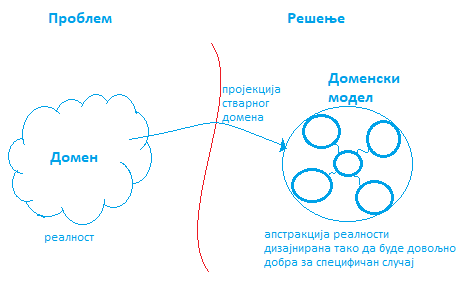
\includegraphics[scale=0.7]{slike/domen-model-projekcija.png}
  \caption{Пројекција реалног домена на једну његову апстракцију}
  \label{fig:domenmodelprojekcija}
\end{figure}
\subsection{Имплементациони обрасци за доменски модел}
Уколико се посматрају слојевите архитектуре софтвера, слој домена би представљао срж апликације. Он изолује сложеност доменског модела од сложености разних техничких делова софтвера. Његова улога је да осигура да се техничке ствари попут логике за управљање трансакцијама, складиштења података и приказивања не умешају у сложеност доменске логике. Мешањем инфраструктурне и доменске логике добија се кôд који је тежи за разумевање, јер има више од једног задужења, и тешко је фокусирати се на само једну ствар. Слој домена обично представља само мали део целокупне апликације, што се може видети на слици \ref{fig:slojevitaarhitektura}.

\begin{figure}[!ht]
  \centering
  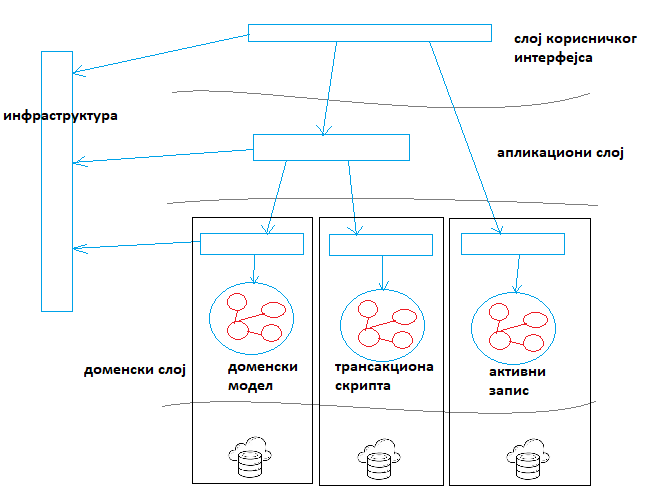
\includegraphics[width=\textwidth]{slike/slojevita-arhitektura.png}
  \caption{Слој домена као део сложеније архитектуре}
  \label{fig:slojevitaarhitektura}
\end{figure}

Конструкција доменских модела је проблем који нема јединствено решење, али у пракси постоје одређена решења, односно имплементациони обрасци, који су општеприхваћени и углавном су се добро показали. Неки од њих више одговарају сложенијим поддоменима, док се други могу искористити код једноставнијих, за прављење простијих и сиромашнијих модела. Популарнији обрасци који се користе су доменски модел (енг.~\textit{domain model}), трансакциона скрипта (енг.~\textit{transaction script}) и активни запис (енг.~\textit{active record})\cite{peaa}.

\paragraph{Образац "доменски модел"}
Овај образац се најбоље уклапа у сложене домене са богатом пословном логиком, и подразумева креирање објектно-оријентисаног модела који садржи податке, пословне процесе и правила, и богату доменску логику. У терминима објектно-оријентисаних програмских језика, ово подразумева креирање класа са потенцијално сложеним међусобним односима, где ће методи садржати доменску логику, поља ће представљати доменске податке, а саме класе ће представљати појединачне ентитете модела који се развија.

Премиса обрасца је да не постоји база података, и да током еволуирања модела проблем складиштења података буде занемарен. Објекти у добијеном моделу су у потпуности ослобођени од инфраструктурних проблема, што омогућава да дизајн модела буде фокусиран искључиво на домен. Ова независност се постиже тако што се у оквиру доменског слоја дефинишу интерфејси за комуникацију са компонентама из нижих слојева. Компоненте из нижих слојева морају да имплементирају дефинисане интерфејсе, чиме се зависност усмерава од ових компоненти ка апстрактнијем доменском слоју. Доменски слој све инфраструктурне услуге користи коришћењем дефинисаних интерфејса над којима има потпуну контролу, уместо да директно комуницира са конкретним компонентама. На слици \ref{fig:razdvajanjedomenskogsloja} се може видети како је доменски слој раздвојен од техничких ствари попут складиштења података.

Ослобађањем доменског слоја од инфраструктурне логике се добија модел који ће се мењати само када се промене пословна правила и процеси. Промене компоненти изван овог слоја немају утицај и не могу нарушити исправност и организацију унутар доменског слоја.

\begin{figure}[!ht]
  \centering
  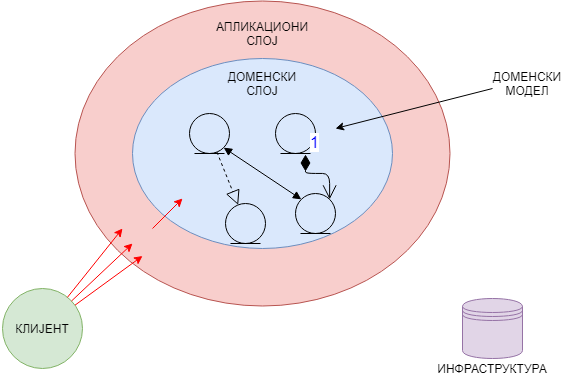
\includegraphics[scale=0.6]{slike/razdvajanje-domenskog-sloja.png}
  \caption{Раздвајање доменског слоја од остатка апликације}
  \label{fig:razdvajanjedomenskogsloja}
\end{figure}

\paragraph{Образац "трансакциона скрипта"}
Трансакциона скрипта је, за разлику од доменског модела, заснована на процедуралном стилу развоја, лакша је за разумевање и имплементацију. Идеја је да се за сваки случај употребе креира по једна процедура, и да се све те процедуре групишу на једно место. Свака од процедура треба да садржи сву логику потребну да се обави одговарајући случај употребе, укључујући ствари попут пословних правила, логике за складиштење података, итд. Предност овог обрасца су једноставност и могућност да се лако имплементирају нови случајеви употребе додавањем нове процедуре, без бојазни да ли ће бити утицаја на постојећу функционалност. Мане су потенцијално много понављања исте логике на различитим местима и лоша подела одговорности. Овакав образац је најприхватљивији за једноставније поддомене који садрже мало логике.

\paragraph{Образац "активни запис"}
Активни запис је популарни образац који подразумева да се сваки објекат модела пресликава у одговарајући ред неке табеле. Погодан је у случајевима када модел базе података одговара доменском моделу, па се може употребити у комбинацији са гореописаним обрасцем "доменски модел" за попуњавање и трајно складиштење доменских података уколико су добијени модели једноставни.

Ова структура ће у себи садржати податке и понашање, као и додатне методе за складиштење, додавање нових инстанци и претраживање колекције објеката. С обзиром да свака од структура има методе за креирање, читање, ажурирање и брисање, могуће је коришћење алата и скриптова за аутоматско генерисање доменског модела. Једна од популарних имплементација овог обрасца је Eloquent ORM која је део PHP развојног оквира Laravel \cite{Laravel}.

\subsection{Ограничени контексти и интегритет доменских модела}\label{ogranicenikonteksti}
Већ је поменута битност разбијања главног домена на неколико мањих. Као резултат тог процеса настају једноставнији поддомени са бољом поделом одговорности, и њихови одговарајући модели; како би се остварила функционалност система, неопходно је да постоји нека интеракција између тих модела. Кључно је да модели буду што независнији, и да ова интеракција буде добро дефинисана. У супротном, лако долази до преплитања концепата и логике из различитих поддомена. Да би се заштитио интегритет модела, дефинишу се јасне границе између различитих модела, а то се постиже везивањем модела за одређени контекст, тзв. ограничени контекст.

За разлику од поддомена, који је апстрактан појам, ограничени контексти представљају конкретну техничку имплементацију која ће форсирати одржање граница између модела апликације. Имплементирају се тако да поседују читав стек (енг.~\textit{stack}) функционалности једног поддомена, укључујући презентациони слој, доменску логику и инфраструктуру. Избор архитектуралног обрасца, па и самих технологија за имплементацију једног контекста се може разликовати од контекста до контекста. Сама филозофија не ограничава избор архитектуре, али је потребно да она буде у стању да изолује доменску логику, јер ће се презентација, инфраструктура и доменска логика мењати различитим интезитетом, и из различитих разлога. Један од архитектуралних образаца који омогућава ову изолацију је слојевита архитектура, описана у секцији \ref{sectionslojevitaarhitektura}.

Контексти се дефинишу на начин који би омогућио поделу послова између различитих тимова, и тако да унутар једног контекста нема двосмислених појмова који би увели забуну. Природно је да за један ограничени контекст буде задужен само један тим, унутар којег би се развијао заједнички језик. С обзиром да су ограничени контексти доста независни, и комуникацију са другим контекстима обављају преко јасно дефинисаних интерфејса, један тим би јако мало зависио од других тимова, и њихови рокови дистрибуције нових верзија софтвера не би зависили од другог тима и њихових проблема. Ово важи све док се не наруши компатибилност променом интерфејса преко којих се комуникација обавља.

\section{Слојевитe архитектурe}\label{sectionslojevitaarhitektura}
У претходној секцији је речено да архитектурални стил сваког појединачног ограниченог контекста мора да подржи раздвајање доменске логике од осталих делова, односно раздвајање одговорности. Да би се ово постигло, могу се креирати различити слојеви у оквиру ограниченог контекста, где би сваки слој био задужен за неку од одговорности. На слици \ref{fig:inverzijazavisnosti} се може видети слојевита архитектура са доменским слојем у самом језгру. Доменски слој је у потпуности ослобођен било каквих зависности, и фокусиран је искључиво на доменску логику. Апликациони слој који окружује доменску логику има улогу да имплементира случајеве употребе, и то тако што ће управљати доменским моделима и делегирати захтеве доменском слоју. Једина зависност коју апликациони слој треба да има је зависност од доменског слоја.

Ова два слоја ће имати потребу за складиштењем података, и за разним другим инфраструктурним услугама. Да би се ово остварило без увођења додатне зависности, примењује се принцип познатији као инверзија зависности (енг.~\textit{dependency inversion}). Инверзија зависности у овом случају подразумева да, уместо да се апликациони слој прилагођава специфичностима сваке инфраструктурне услуге, свака од услуга имплементира унапред дефинисан интерфејс од стране апликационог слоја. Додатна корист од независности апликационог и доменског слоја од остатка је њихово олакшано тестирање, тј. тестирање доменске логике у изолацији, без инфраструктурних зависности.
\begin{figure}[!ht]
  \centering
  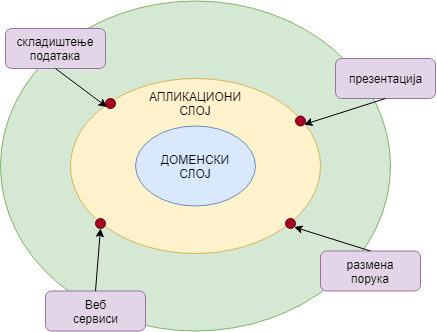
\includegraphics[scale=0.7]{slike/inverzija-zavisnosti.png}
  \caption{Слојевита архитектура апликације са инверзијом зависности}
  \label{fig:inverzijazavisnosti}
\end{figure}
\section{Интеграција ограничених контекста}\label{integracijaogranicenihkonteksta}
Сваки од ограничених контекста може представљати засебан процес који може бити извршаван на различитим физичким машинама. Добра ствар овог приступа где су различити контексти засебни процеси је то што је апликација отпорнија на отказивање одређених компоненти система, па чак и на саме физичке кварове. Додатно, софтвер је скалабилнији. У случају повећаног броја корисника, а самим тим и количине операција које апликација обрађује, софтвер мора бити у стању да се скалира како би успешно опслужио све кориснике.

Једно од решења је вертикално скалирање, које подразумева повећање хардверских ресурса на једној машини, попут радне меморије, складиштног простора, и броја процесора. Овај приступ има ограничење, и повећање ресурса на тај начин не може бити дугорочно решење. Боље решење је да апликација буде способна да се скалира хоризонтално, односно, да се са порастом оптерећења система додају нове физичке машине у инфраструктуру, и да се покрећу додатне инстанце софтвера. Међутим, по правилу су овакви системи доста сложенији; уместо једне монолитне апликације постоји више дистрибуираних процеса који међусобно морају да сарађују и комуницирају, најчешће посредством рачунарске мреже. Потребно је дефинисати на који начин ће те компоненте бити интегрисане, како ће се синхронизовати, а јавља се и питање конзистентности. Сви наведени проблеми представљају нешто са чиме се сваки дистрибуирани систем суочава, и од система до система се могу разликовати реализована решења, а у зависности од случајева употребе, природе самог домена, и очекивања корисника.

Нека од конкретних техничких решења која могу бити употребљена за комуникацију унутар оваквог система су интеграција помоћу датотека, интеграција коришћењем базе података,  позив удаљене процедуре (енг.~\textit{remote procedure call}), интеграција коришћењем система за размену порука (енг.~\textit{messaging}) и REST интерфејси за програмирање апликација. Архитектура система који се креира би требало да буде таква да нуди могућност одлагања одлуке о интеграцији што дуже, односно, требало би да буде флексибилна у смислу да један вид интеграције у току развоја може бити замењен другим, без утицаја на доменски слој, и уз што мање утицаја на друге слојеве.

\subsection{Интеграција помоћу датотека}
Интеграција помоћу датотека представља један од најједноставнијих видова интеграције ограничених контекста који подразумева да једна компонента упише нешто у датотеку, а да онда друга компонента то прочита. Ово читање би могло да буде имплементирано тако да компонента која чита то ради на сваких неколико секунди или минута. Иако је ово решење доста флексибилно у погледу формата и организације података, поседује и неке мане због којих је прихватљиво употребити га само у некритичним деловима система или у првобитним итерацијама. Ту се пре свега мисли на проблеме са скалирањем, редудантношћу и синхронизацијом података.

Уколико се овакав тип интеграције користи као дугорочно решење, потребно је имплементирати механизам који решава наведене проблеме. Ово може бити скупо и захтевно за имплементацију, подложно грешкама и било би тешко постићи перформансе готових софтверских решења. Решење је прихватљиво за компаније које већ имају имплементиран овај механизам као готов и добро тестиран производ.

\subsection{Интеграција коришћењем базе података}
Овај тип интеграције је доста сличан интеграцији помоћу датотека. Уместо да део апликације податке уписује у датотеку, може их уписати у неку базу података, из које касније друга компонента може да чита. 

Један проблем који се јавља код оваквог типа интеграције је то што су компоненте спрегнуте са базом података. Уколико једна компонента има захтев за променом схеме базе података, друга компонента би морала да се прилагоди тој новој схеми. Додатно, код база података као потенцијални проблем се јавља и закључавање које се поприлично може одразити на перформансе уколико један део апликације нпр. интезивно уписује у базу, а други део врши ажурирање. Поред тога, код овакве интеграције база је критична тачка пуцања. Уколико база није доступна, комуникација између компоненти ће бити онемогућена.

Иако је овај начин интеграције поузданији и решава озбиљне проблеме интеграције помоћу датотека, оно и даље представља примитивно решење које би требало употребити само у првобитним итерацијама или у некритичним деловима система. Уколико се база података користи као привремено решење, и користи се само за интеграцију, у том случају је пожељније користити интеграцију помоћу датотека, чиме се избегавају додатна подешавања базе података. У наставку ће бити описани флексибилнији и скалабилнији начини интеграције.

\subsection{Позив удаљене процедуре}
Позив удаљене процедуре је популаран и често коришћен начин интеграције. У основи, комуникација између две компоненте се обавља посредством рачунарске мреже, коришћењем неког протокола, најчешће HTTP. Идеја је да се од програмера прикрије чињеница да су компоненте физички удаљене, и да се комуникација одвија преко мреже. Летимичним погледом на кôд се не може закључити да се ради о мрежној апликацији, јер је сама сложеност мрежне комуникације скривена, а позиви метода, као и њихова имена ни на који начин не откривају да се не ради о монолитној апликацији. У позадини, ово се изводи тако што се за методе које представљају удаљене процедуре генерише клијентски и серверски кôд. Он између осталог садржи логику за серијализацију и десеријализацију параметара и позиве мрежних функција. Позив метода у клијентској апликацији проузрокује да се порука са информацијом о методу који се позива и листом параметара серијализује у низ бајтова, и онда се шаље кроз мрежу. На серверској страни се порука прима, десеријализују се назив метода и његови параметри, и извршава се одговарајући удаљени кôд. Транспарентност овог начина интеграције уједно може бити и његова мана. Врло је лако заборавити да се ради о мрежним позивима, па њихово неоптимално и пречесто позивање може довести до проблема са перформансама. Такође, позиви удаљених процедура су проблематични уколико постоји захтев да се неки кôд извршава асинхроно. У том случају, боље решење представља коришћење система за размену порука.

\subsection{Интеграција коришћењем система за размену порука}
Интеграција коришћењем система за размену порука се користи у апликацијама чије би компоненте требало да комуницирају асинхроно. Систем за размену порука је најчешће имплементиран као дистрибуирани ред који има могућност да се скалира, реплицира податке и шаље их кроз мрежу, и може се посматрати као засебна компонента. У односу на позив удаљених процедура, овај метод интеграције је отпорнији на отказивање компоненти, јер савремени системи за размену порука имају могућност чувања порука које нису послате, у случајевима када постоје мрежни проблеми, или уколико компонента која прима поруке привремено није активна, као и поновно слање тих порука када је систем поново стабилан. Када нека компонента жели да шаље поруке, шаље их у виду догађаја (енг.~\textit{events}), заједно са додатним подацима неопходним за обрађивање тог типа догађаја. Компоненте заинтересоване за одређени тип догађаја се могу претплатити (енг.~\textit{subscribe}) на исти. На овај начин компонента која врши слање уопште не мора да зна ко све прима поруку, већ ће компоненте које желе да обрађују одређени тип догађаја претплатом изразити интересовање. Мана овог приступа је то што се подразумева употреба асинхроне парадигме, која је скоро увек захтевнија за имплементацију и разумевање јер се доста разликује од конвенционалног синхроног програмирања. Такође, захтева посматрање проблема из другачијег угла, као и сасвим другачији дизајн компоненти.

\subsection{REST интерфејси за програмирање апликација}
REST интерфејси су интерфејси за програмирање апликација који су имплементирани у складу са REST архитектуралним стилом и омогућавају комуникацију са удаљеним сервисима. Дизајнирани су тако да могу да искоришћавају постојеће протоколе и због тога није неоподна инсталација додатних библиотека и додатног софтвера. Најчешће се користи HTTP, али у теорији се може користити било који протокол. Неки од критеријума које интерфејс мора да задовољи да би био у складу са REST архитектуралним стилом су:
\begin{enumerate}
\item клијентско-серверска архитектура која се састоји од клијената, сервера и ресурса;
\item комуникација између клијената и сервера је без стања, односно, сервери не чувају информације о клијентима између различитих захтева (непостојање сесије);
\item сваки ресурс мора бити јединствено идентификован, и њихова интерна репрезентација треба бити раздвојена од репрезентације која се шаље клијентима;
\item репрезентација ресурса коју добија клијент мора да садржи довољно информација које ће омогућити управљање самим ресурсом, као и довољно информација о томе како би клијент требало да процесира поруку;
\item коришћење хиперлинкова у одговору који би референцирали друге повезане ресурсе.
\end{enumerate}
Централни појам REST архитектуре је ресурс. Ресурсом се може сматрати практично све што је довољно важно да буде референцирано; то су најчешће ствари које могу бити складиштене у рачунарима, попут електронских докумената, редова у базама података и резултата неког алгоритма. Услов који мора да задовољи сваки ресурс је да има свој јединствени идентификатор URI (енг.~\textit{unique resource identifier}) на основу којег ће бити референциран \cite{RESTfulWebAPIs}. Називи ресурса би требало да буду именице, а не глаголи; у фокусу архитектуре су ресурси, а не процедуре. Добри кандидати за ресурсе су поддомени који су добијени анализом и разбијањем проблема, као и независни ентитети који представљају део модела тих поддомена.

Ресурси се организују логички у хијерархије. Хијерархија се успоставља угнежђавањем имена ресурса у URI идентификатору. Име ресурса који је хијерархијски ниже у односу на неки други ресурс се у јединственом идентификатору појављује касније. Оваквим приступом се јасније осликава однос међу ресурсима; нпр. идентификатор \textit{/knjige/[id knjige]/recenzije/[id recenzije]} јасније говори о односу ентитета "књига" и "рецензија" него два одвојена идентификатора \textit{/knjige/[id knjige]} и \textit{/recenzije/id recenzije}. Други разлог за овакву организацију је зависност неких ресурса од контекста у којем се налазе; у идентификатору \textit{/ulice/[naziv ulice]/kuce/[broj kuce]} број куће је локалан у односу на улицу у којој се налази.

Комуникација међу сервисима се одвија разменом репрезентација ресурса. Битно је напоменути да сам ресурс и његова репрезентација не представљају исту ствар. Репрезентација ресурса је стање ресурса представљено на користан начин, у одређеном формату. Формат који се користи за репрезентацију није дефинисан самим архитектуралним стилом, и може се користити формат по избору. Најчешће се користе JSON (енг.~\textit{JavaScript Object Notation}) и XML (енг.~\textit{eXtensible Markup Language}), због њихове једноставности, флексибилности и доступности великог броја различитих имплементација рашчлањивача (енг.~\textit{parser}).

Поред појединачних ресурса, могуће је конструисати и скупове ресурса истог типа, односно колекцију ресурса. Сама колекција, и сваки од њених елемената има свој јединтвени идентификатор. Дохватањем репрезентације колекције, враћа се листа репрезентација објеката који се у њој налазе. Добра пракса је да се за сваки елемент колекције прикаже мининална репрезентација, уз хиперлинк који ће водити ка детаљној репрезентацији. Такође, требало би омогућити и филтрирање елемената колекције на основу различитих параметара, како би се сузио скуп елемената на неки одређени подскуп. У случају великих колекција, потребно је увести пагинацију којом би се ограничио број елемената који се враћа једним одговором.   

\subsubsection{Креирање захтева}
Управљање удаљеним ресурсима се врши формирањем захтева у одређеном формату где се наводи јединствени идентификатор ресурса, глагол који описује каква операција се врши над ресурсом, и додатни атрибути који описују остале специфичности које се односе на операцију која се извршава. Операције за управљање се могу поделити у две групе: оне које мењају стање ресурса, и оне које не мењају. Мењање ресурса подразумева мењање стања постојећих ресурса, додавање нових и брисање постојећих ресурса.

Уколико се за комуникацију користи HTTP протокол, креирање захтева подразумева попуњавање заглавља и тела HTTP поруке. У заглављу се наводи URL ресурса, а глагол који описује операцију може бити један од предефинисаних глагола у склопу протокола (GET, POST, PATCH, DELETE, PUT). Обрада захтева се имплементира тако да се поштује семантичко значење глагола који се шаље у захтеву. Нпр. GET би било неприродно користити за све осим за дохватање репрезентације ресурса, и било би очекивано да такав захтев не мења стање. Додатне информације које се прослеђују кроз захтев се наводе додавањем HTTP атрибута и попуњавањем тела HTTP поруке.

Семантичка значења HTTP глагола су следећа:
\begin{enumerate}
\item GET --- дохвата репрезентацију удаљеног ресурса који је референциран његовим јединственим идентификатором, без мењања стања ресурса;
\item POST --- креира нове ресурсе, али се може користити и за акције које мењају стање, али не стварају нове ресурсе;
\item PATCH --- мења постојећи ресурс новим ресурсом;
\item DELETE --- брише ресурс референциран јединственим идентификатором;
\item PUT --- мења стање постојећих ресурса.
\end{enumerate}

\subsubsection{Формат одговора}
Одговор на одређени захтев треба да садржи информацију о статусу извршене операције. Додатно може садржати и репрезентације ресурса, као и хиперлинкове ка повезаним ресурсима. За статус захтева код HTTP протокола се користе постојећи статусни кодови који су дефинисани стандардом. Као и глаголи, кодови се користе тако да поштују њихово семантичко значење.

\chapter{Микросервисна архитектура}\label{mikroservisi}
Микросервиси представљају архитектурални стил којег одликују мали, независни сервиси који раде заједно како би обавили неки посао. Због сличности, неретко долази до мешања термина микросервиса и доменски оријентисаног моделовања. Та сличност потиче од чињенице да доменски оријентисано моделовање представља само филозофију развоја, односно скуп препорука, образаца и циљева, док су микросервиси једно конкретно решење како се та филозофија може применити у стварности.

Употреба доменски оријентисаног моделовања у микросервисној архитектури се огледа у подели апликације на мале, добро дефинисане сервисе праћењем смерница за разбијање домена на поддомене, образаца за моделовање добијених поддомена и применом стратегија за интеграцију резултујућих сервиса; ове смернице, обрасци и стратегије су описане у оквиру поглавља \ref{domenskiorijentisanomodelovanje}. Оно што микросервисну архитектуру чини јединственом у односу на друге архитектуралне стилове који такође врше поделу система на сервисе је гранулација сервиса, односно њихова величина, као и оријентисаност сервиса ка домену проблема. Дизајн система моделованог коришћењем доменски оријентисаног моделовања ће садржати ограничене контексте, и управо су ови контексти природне границе сервиса \cite{netmicroservices}. Ограничени контексти су обрађени у секцији \ref{ogranicenikonteksti}.

Скоро сва комуникација се одвија преко мрежних позива, који су скупе операције, и форсира се што већа раздвојеност међу сервисима; на тај начин се смањује опасност од велике спрегнутости. Независност и мала спрегнутост омогућавају да се мењање једног сервиса и дистрибуција нових верзија обављају независно у односу на остале сервисе.

Сваки сервис дефинише интерфејс за програмирање апликација преко којег остали сервиси могу да комуницирају са њим. Раздвојеност сервиса програмерима даје слободу да користе различите програмске језике у различитим сервисима, па технологија која се користи за интерфејс треба да буде језички неутрална (енг.~\textit{language-agnostic}), односно да не ограничава избор програмског језика \cite{BuildingMicroservices}. Поред коришћења различитих програмских језика, различите компоненте такође могу да користе и различите механизме за трајно складиштење података. На пример, један сервис може да буде имплементиран у програмском језику C++ и да користи релациону базу података, а неки други може да буде имплементиран у Пајтону (енг.~\textit{Python}) и да за складиштење користи обичну датотеку. Предност овога је то што се избор технологије може вршити у зависности од природе поддомена и потребних перформанси, преференција особе или тима задуженог за одређени сервис, и слично. Додатно, мање битни сервиси могу да експериментишу са новим технологијама, без страха да ће се евентуални проблеми прелити на остатак система. И наравно, пошто су сервиси мали, врло је лако поново их имплементирати у неком другом програмском језику уколико коришћена технологија не испуни очекивања.   

\section{Предности и мане}
С озбиром да се ради о независним сервисима, јасно је да микросервиси потпадају у категорију дистрибуираних система. Самим тим наслеђују њихове предности и мане. Неке од предности дистрибуираних система су редудантност и отпорност на отказивање, боље скалирање и бржи одзив. Ипак, иако због свега овога звуче као добро решење за сваки проблем, микросервиси имају и отежавајуће околности довољно велике да није исплативо користити их уколико природа самог проблема који се решава не захтева то. Пре свега, ту се мисли на безбедност, проблеме са конзистентношћу и теже детектовање проблема.

\subsection{Редудантност и отпорност на отказивање}
Ова секција започиње поређењем отпорности на отказивање монолитних апликација у односу на микросервисе. Уколико један модул монолитне апликације услед неког проблема откаже, нпр. референцирањем показивача на невалидну меморијску локацију, цела апликација насилно завршава са извршавањем. Такође, ако дође до отказивања физичке машине, једна једина инстанца апликације са којом је корисник имао интеракцију престаје да постоји. Укратко, отпорност на овакве врсте отказа не постоји.

За разлику од монолитне апликације, отказивање једног сервиса у микросервисној архитектури не утиче на доступност осталих сервиса, било да се ради о отказивању сервиса услед неке грешке, или о отказивању физичке машине (ово важи ако се сви сервиси не налазе на истој машини). Један од начина како се микросервисна архитектура бори са оваквим проблемима је да након отказивања систем може да пређе у другачији режим рада, са редукованим функционалностима док се проблематични сервис поново "не подигне".

Други начин је постојање резервних (енг.~\textit{backup}) инстанци које би могле да замене инстанцу која више није активна. Резервне инстанце могу бити активне и у стању приправности све време у току рада примарне инстанце, a могу бити и искључене, и покренуте по потреби; то је тзв. хладна резерва (енг.~\textit{cold backup}). Хладна резерва се користи у ситуацијама кад је подизање сервиса брзо, или је период неактивности док се сервис подиже прихватљиво. Предност хладних резерви је у томе што примарни и резервни сервиси нису активни истовремено, па самим тим утрошак ресурса није дупло већи.

Било да се користе активне или хладне резерве, потребно је да постоји механизам који може да утврђује да ли је примарна инстанца активна или није, и да ли је у стању да обрађује захтеве, и да покреће резервне инстанце уколико је потребно. Овај механизам мора радити поуздано, како би се избегла ситуација где и примарна и резервна инстанца активно прихватају и обрађују захтеве; таква ситуација је опаснија од тоталне неактивности, јер може нарушити стање целог система. Једно од софтверских решења које се користи у ове сврхе је Apache ZooKeeper \cite{Zookeeper}.

\subsection{Скалирање}
У секцији \ref{integracijaogranicenihkonteksta} је назначено да постоје два типа скалирања - хоризонтално и вертикално; наведени су и разлози зашто се преферира хоризонтално скалирање у односу на вертикално. Код поддомена који су по природи погодни за паралелизацију постоји могућност покретања више инстанци истог сервиса како би се оптерећење са једне инстанце једнако распоредило на више њих. Број инстанци једног сервиса се мења динамички, односно, у току већег налета захтева ка систему, покрећу се додатне инстанце како би се избегло оптерећење и успорена обрада података. Када се број захтева врати у нормалу, додатне инстанце се искључују. Ово додавање и избацивање инстанци се може обављати ручно, али може бити и аутоматизовано, тако што ће се број инстанци регулисати на основу статистике, нпр. на основу броја активних корисника, захтева у секунди, одзива и слично. Једна од најбитнијих ствари које корисници система очекују је то да добијају одговоре на њихове захтеве у што краћем року.

\subsection{Одзив}
У претходној секцији је речено да је одзив јако битна карактеристика која може утицати на задовољство корисника. Ово не зависи увек само од оптерећења система, већ и од тога где су корисници географски лоцирани у односу на сам систем. Систем може бити растерећен, али уколико је корисник на другом крају света, спорији одзив услед пропагације података кроз мрежу се не може избећи. Ово се решава тако што се покреће више инстанци истог сервиса, али на различитим локацијама широм света. Балансери захтева на основу локације корисника онда могу да одаберу физички најближи сервис са којим ће корисник комуницирати.

\subsection{Безбедност}
Током развоја софтвера је изузетно битно да се пажња обрати и на безбедност, посебно уколико се ради о софтверу високог значаја\footnote{Ово подразумева софтвер који ради са личним подацима људи, обавља критичне операције које могу утицати на људске животе у економском или здравственом смислу, и било који други софтвер који ради са подацима који се сматрају поверљивим, попут државних тајни, итд.}. Дистрибуирани системи за комуникацију интезивно користе рачунарске мреже, што ствара додатне слабе тачке које је потребно заштитити. Поред стандардних пропуста који се јављају код једнопроцесних апликација, рачунарске мреже отварају нове могућности за искоришћавање система у сврхе које су изван дефинисаних случајева употребе, међу којима су и оне малициозне. Главна линија одбране би требало да буде добро подешена мрежа која би спречила евентуалне упаде уљеза, али и поред тога, сва комуникација међу сервисима би требало да се одвија као да ће потенцијални уљези пробити заштитну баријеру мреже. То подразумева пажљиво и детаљно обрађивање корисничких захтева; додатно, већина саобраћаја (ако не и сав саобраћај) би требало да буде енкриптована, посебно део комуникације који може садржати осетљиве податке, попут лозинки, бројева картица, и слично.

Код дистрибуираних система код којих су перформансе од великог значаја, посебно код система који раде у реалном времену, енкрипција података може представљати проблем. Криптографске функције могу створити додатни утрошак (енг.~\textit{overhead}) драгоцених ресурса, посебно уколико се користе јачи алгоритми за енкрипцију. У том случају, уместо шифровања свих података у систему, могу се шифровати само осетљиви подаци, као и комуникација између клијената и самог система.

\subsection{Конзистентност}
Постојањем више раздвојених сервиса, добијају се бољи одзив и скалирање, и апликација је отпорнија на отказивање, али се јављају проблеми са конзистентношћу. Конзистентност подразумева да захтев за неким подацима ка било којем сервису унутар система увек враћа најсвежије податке. Пропагација података кроз цео систем захтева одређено време, и јасно је да решење овог проблема не може бити савршено, већ мора постојати неки компромис. Ово тврђење је део познате CAP (енг.~\textit{consistency - availability - partition tolerance}) теореме која каже да је немогуће обезбедити истовремено задовољење конзистентности, расположивости и толеранције раздвојености, и постоји математички доказ који потврђује ову теорему \cite{10.1145/564585.564601}. Толеранција раздвојености подразумева да систем мора бити у стању да прихвата делимичне отказе и наставља да ради исправно.

\subsection{Надгледање}
Надгледање софтвера (енг.~\textit{monitoring}) у продукцији и детектовање евентуалних проблема је изузетно важан процес. Информациони системи од великог значаја не трпе дуготрајне периоде неактивности, и све потенцијалне проблеме је потребно детектовати на време, и одреаговати што пре. Код монолитних апликација, овај задатак је релативно праволинијски, и подразумева праћење логова, надгледање живости и "здравља" саме апликације, и то најчешће може бити аутоматизовано. Код микросервиса је ово мало сложеније, због многобројних сервиса које је потребно пратити. Истовремено је потребно пратити стање свих активних инстанци сервиса у систему, на различитим физичким и виртуелним машинама, и овде је аутоматизација неопходна; свако друго решење је непродуктивно. Ручно праћење логова и проверавање појединачних сервиса би захтевало много времена и велики фокус. Додатно, поред "здравља" појединачних сервиса, потребно је обратити пажњу и на стање мреже која омогућава комуникацију и сарадњу сервиса. Да би се овај задатак аутоматизовао, мора постојати механизам откривања сервиса (енг.~\textit{service discovery}) који може да детектује динамичне промене у инфраструктури, попут додавања нових инстанци и њиховог уклањања.

\section{Упошљавање софтвера}
Упошљавање софтвера (енг.~\textit{deployment}) представља све активности које је неопходно обавити како би се апликација оспособила за употребу. То укључује дистрибуцију нове верзије, инсталацију, подешавање, деинсталацију и ажурирања. Ситне промене у сложеним монолитним апликацијама захтевају да се изврши упошљавање целе апликације. Упошљавање велике апликације представља процедуру која носи огроман ризик, па се у пракси овако ризичне процедуре дешавају што је ређе могуће; пре упошљавања се обично скупи доста измена, које се онда дистрибуирају кроз исту верзију. У међувремену су корисници могли да промене мишљење и да одлуче да ипак не желе неку функционалност, или су одлучили да желе да нешто функционише другачије. Услед нагомиланих измена, теже је селективно поништити само неке од измена, посебно јер можда те измене зависе од неких других.

Код микросервиса је прича једноставнија. Сервис у којем су направљене измене се може распоредити независно од осталих сервиса у систему. Лакше се поништавају направљене измене у случају проблема, а и сам проблем је изолован од остатка система. Такође, нове измене се дистрибуирају много брже. Ипак, због постојања више независних сервиса, односно више независних мини пројеката, систем за изградњу (енг.~\textit{build system}) и верзионисање софтвера је сложенији; додатно, теже је пратити колико инстанци сервиса имамо, и где се све они налазе. Услед непажње, није немогуће заборавити на неки сервис током упошљавања, и зато, ова процедура би требало да буде аутоматизована.

\subsection{Хостовање сервиса}\label{hostovanjeservisa}
Речено је да сваки од сервиса може да се извршава независно, и према томе, сваки од њих се може налазити на различитим машинама. У екстремном случају, сваки сервис може имати своју засебну машину, чиме се постиже велика отпорност на отказивање, и сваки сервис је максимално изолован, с обзиром да су му сви ресурси машине и оперативног система на располагању. Међутим, ово није увек најбоље решење када је у питању искоришћеност ресурса, а притом није ни исплативо; ако се ради о неким једноставним сервисима, ресурси машине ће бити углавном неискоришћени. Уколико желимо велику изолованост сервиса, постоје и друга могућа решења којима се то може постићи.

Једно од класичних решења је употреба виртуелних машина. Једна физичка машина може имати више виртуелних машина, и свака од њих ће имати свој засебан оперативни систем, и у стању је да пружи велики ниво изолације микросервисима. По потреби се могу покретати нове инстанце машина, и гасити постојеће, што даје већу флексибилност него код решења са једном физичком машином по сервису. Ово решење је сасвим прихватљиво, али свака од виртуелних машина хостује по један оперативни систем у целости, и тиме се ствара поприличан додатни утрошак ресурса на гостујуће оперативне системе (енг.~\textit{guest operating system}).

Друго решење је употреба све популарнијих софтверских контејнера, који попут виртуелних машина могу изоловати сервисе од остатка система. И они такође врше одређени степен виртуелизације, али не постоји више инстанци оперативних система, и њихов додатни утрошак је далеко мањи од утрошка који стварају виртуелне машине. Остале предности контејнера у односу на виртуелне машине су:
\begin{enumerate}
\item величина --- с обзиром да контејнери не садрже комплетан оперативни систем, њихова величина се може мерити десетинама мегабајта, што значи да се изузетно брзо могу реплицирати и копирати са једне физичке машине на другу;
\item брзина креирања и реплицирања --- због природе контејнера, њихово креирање, реплицирање и уништавање су изузетно ефикасне операције, што погодује великој динамичности дистрибуираних система - могуће је подизање нових инстанци сервиса за свега неколико секунди.
\end{enumerate}
Један пример технологије софтверских контејнера је Докер \cite{Docker}, који је широко распрострањен у сервисно оријентисаним архитектурама, јер омогућава лако покретање контејнера на инфраструктурама у облаку (енг.~\textit{cloud infrastructure}).

\section{Тестирање}
Тестирање је неизоставан део било које методологије развоја софтвера, и једнако је важно колико и сам процес имплементације. Улога тестирања у развоју је стицање што веће поузданости у исправност софтвера који се развија. Обично није могуће достићи стопроцентну поузданост, али је могуће открити велики број функционалних и нефункционалних недостатака. Од покривености различитих случајева употребе, специјалних случајева и методологије тестирања зависи колико ће тестови добро обављати свој посао. Када говоримо о тестирању микросервиса, једна могућа класификација тестова је на јединичне тестове, тестове појединачних сервиса и тестирање интеграције сервиса, познатије као тестирање с краја на крај (енг.~\textit{end-to-end tests}).

\subsection{Јединично тестирање}
Јединично тестирање подразумева проверу исправности малих логичких целина (обично је то тестирање појединачних функција) од којих је сервис изграђен. Ове логичке целине треба да буду изоловане од остатка сервиса, а све зависности би требало заменити примитивним и лажним (енг.~\textit{mock}) зависностима. Од свих наведених врста тестова, ови тестови су најбржи, требало би да их има највише, и да процентуално детектују највише грешака. Обично су аутоматизовани, и неизоставни су део непрекидне интеграције софтвера (енг.~\textit{continuous integration}) која подразумева што чешће "комитовање" (енг.~\textit{commit}) измена, изградњу након сваке измене и покретање аутоматских тестова.

\subsection{Тестирање појединачних сервиса}
Тестирање појединачних сервиса има улогу да провери исправност читавог сервиса, односно функционалности које сервис пружа, и то преко јавног интерфејса који је изложен. Исправност мањих логичких целина је покривена јединичним тестовима, а овај тип тестова би требало да провери да ли су те целине исправно интегрисане. И ове тестове је углавном могуће аутоматизовати. Нешто су спорији од јединичних тестова јер покривају логички веће целине, и количински их има мање.

\subsection{Тестирање с краја на крај}
Претходна два типа тестирања су тестирања која се примењују и код монолитних апликација. Пошто се сервисне архитектуре састоје од више независних компоненти које међусобно сарађују, потребно је увести још један тип тестирања који би проверавао исправност система који се добија интеграцијом припадајућих сервиса. Ово тестирање се примењује тако што се шаљу различити захтеви, који се пропагирају кроз цео систем, а затим се врши анализа исправности добијеног одговора. Ове тестове је могуће делимично аутоматизовати, креирањем скриптова који би се повремено покретали, и њима је могуће тестирати исправност и перформансе система. Ипак, тестирање безбедности целог система није могуће извршити у потпуности аутоматски, већ се тај део посла обавља ручно, и то обично од стране етичких хакера. Тестирање с краја на крај (енг.~\textit{end-to-end testing}) је најспорије и најзахтевније, па је битно да таквих тестова количински нема превише, и да су изабрани тестови квалитетни и репрезентативни.

\chapter{Имплементација апликације \textit{My Running Buddy}}\label{prakticnideo}
Практични део рада представља конкретан пример примене микросервиса: имплементирана је апликација \textit{My Running Buddy} \cite{implementacija}. Циљ развијене апликације је проналажење одговарајућег партнера за трчање, и намењена је људима који се рекреативно или професионално баве трчањем. Након успешног повезивања два тркача, апликација им омогућава међусобну приватну комуникацију. У оквиру овог поглавља су описане коришћене технологије, као и све најбитније тачке развоја апликације, укључујући алгоритам за упаривање тркача, изазове и неке имплементационе детаље.

\section{Кратак преглед коришћених технологија}
Најпопуларније микросервисне технологије за креирање микросервиса обухватају развојни оквир Spring Boot \cite{SpringBoot} за програмски језик Јава, развојнe оквирe Lumen \cite{Lumen}, Silex \cite{Silex} и Slim 3 \cite{Slim3} за програмски језик PHP, развојни оквир GoMicro \cite{GoMicro} за све популарнији програмски језик Golang и развојни оквир Flask \cite{Flask} за програмски језик Пајтон. За асинхрону комуникацију микросервиса заснованих на догађајима популаран је Apache Kafka \cite{Kafka} дистрибуирани ред, а за синхрону комуникацију REST интерфејси и gRPC \cite{gRPC}. За потребе складиштења податка, најчешће се користе релационе базе података. Неки од популарних система за управљање релационим базама података су Oracle \cite{oracledbms}, MySQL \cite{mysql}, SQL Server \cite{sqlserver} и PostgreSQL \cite{postgresql}.

У овом раду, за имплементацију микросервиса и интерфејса за програмирање апликација коришћени су развојни оквир Lumen за програмски језик PHP, а за складиштење података је коришћен систем за управљање базама података MySQL. За имплементацију клијентске апликације коришћен је Android комплет за развој софтвера, а ауторизација се обавља коришћењем протокола OАuth 2 \cite{MasteringOAuth2}. За потребе тестирања, употребљена је контејнерска технологија Докер, која се такође може користити и у продукционом окружењу.

\subsection{Развојни оквир Lumen}
Lumen је развојни оквир отвореног кода за програмски језик PHP, који се користи за развој микросервиса и интерфејса за програмирање апликација. Имплементира архитектурални стил MVC (енг.~\textit{model-view-controller}), одликује га велика брзина обраде захтева, и тренутно је најбоље решење, с обзиром да се на тестирању перформанси показао боље у односу на конкурентне развојне оквире попут Silex и Slim 3. Lumen представља олакшану (енг.~\textit{lightweight}) верзију популарног PHP развојног оквира Laravel, односно, дизајниран је тако да буде погодан за развој микросервиса.

Сложеност овог оквира долази управо из Laravel компоненти на које се ослања. Ове компоненте су познатије под именом Illuminate, и имплементиране су у складу са унапред дефинисаним интерфејсима, па тако постоје интерфејси за складиштење података, слање мејл порука, и слично. Овај важан принцип је споменут у оквиру секције \ref{sectionslojevitaarhitektura}, где се примењује инверзија зависности како би се избегло увођење инфраструктурних зависности у самој доменској логици. Кључне компоненте су:
\begin{enumerate}
\item компонента за рутирање, чија је улога да све добијене HTTP захтеве повеже са одговарајућом логиком која треба да их обради;
\item компонента средњег слоја (енг.~\textit{middleware}) која се користи за филтрирање захтева који долазе, и на овом слоју се могу радити аутентификација и ауторизација;
\item компонента контролер, унутар које се налази главна логика апликације (апликациони слој) која обрађује захтеве делегирањем операција доменским моделима.
\end{enumerate}

\subsection{Оперативни систем Android}
Android \cite{Android} је оперативни систем отвореног кода који је заснован на модификованој верзији Линукс језгра (енг.~\textit{Linux kernel}). Android је првенствено дизајниран и прилагођен мобилним уређајима и таблетима, мада га све више користе и паметне телевизије. Развијен је од стране удружења програмера Open Handset Alliance које спонзорише Гугл (енг.~\textit{Google}) и лансиран је у јавност септембра 2007. године. Разлози за популарност овог оперативног система су отвореност кода, а самим тим и доступност већој заједници програмера, богато развојно окружење, редукована цена развоја, и привлачно и интуитивно графичко окружење.

Апликације за Android су се дуги низ година развијале у програмском језику Јава, уз коришћење Android комплета за развој софтвера. Овај комплет садржи колекцију софтверских алатки и библиотека неопходних за развој на платформи Android. Уз нове верзије оперативног система се објављује и ажурирани комплет за развој. Велика предност овог оперативног система је то што програмери могу да развију апликацију, а она ће моћи да ради на свим, или скоро свим уређајима које покреће Android\footnote{Да би апликација у потпуности одржала компатибилност са ранијим верзијама оперативног система, потребно је избегавати коришћење нових функционалности које разбијају компатибилност.}. Поред писања апликација у Јави, софтвер је могуће развијати и у програмском језику C++, Пајтону, као и све популарнијем језику Котлин који је сада препоручени језик за развој Android апликација\footnote{С обзиром да је фокус овог рада на микросервисној архитектури, за развој клијентске апликације уместо нове технологије користи се програмски језик Јава са којим је више људи имало додира, чиме би се омогућило лакше праћење и анализа рада широј публици.}. Програмери Android апликација имају могућност да апликацију објаве у оквиру Гугл Плеј продавнице (енг.~\textit{Google Play store}), која представља главни сервис за дистрибуцију софтвера. Сервис корисницима на располагање ставља неколико милиона апликација и игрица различитих категорија, што је такође допринело популарности овог система.

\subsection{Систем за управљање базама података MySQL}
MySQL је систем за управљање релационим базама података који је подржан од стране корпорације Oracle \cite{oracle}. Ради се о софтверу отвореног кода, па се може користити у оквиру пројеката без плаћања накнада, и дозвољено је прављење измена у оквиру изворног кода како би се задовољиле специфичне потребе. Софтвер је компатибилан са различитим платформама, попут UNIX, Linux и Windows оперативних система, и може се користити како на серверским, тако и на десктоп машинама. MySQL је, као и већина других конкурентских система за управљање базама података, дизајниран тако да буде поуздан, скалабилан и брз. Најзаступљенији је код развоја веб сајтова и веб апликација, али се може користити и у склопу софтвера другачије намене. Врло често се користи у комбинацији са програмским језиком PHP, и то је главни разлог зашто је одабран овај систем за управљање базом података, мада развојни оквир Lumen омогућава коришћење различитих система без потребе за изменом постојећег кода.

\subsection{Протокол за ауторизацију OAuth2}
OAuth2 је протокол који омогућава размену информација између две стране на поуздан и безбедан начин. Два најчешћа случаја употребе су oмогућавање пријављивања корисника у апликацију уз помоћ налога са неког другог сервиса, и давање дозвола једном сервису да приступа ресурсима неког другог сервиса у име корисника.

Пре него што буде описано како OAuth2 ради, примером који следи биће приказана мотивација која стоји иза настанка овог протокола. Претпоставимо да одређена апликација има могућност да аутоматски попуни информације о кориснику попут имена, презимена и пребивалишта, и те информације попуњава на основу података са неке друштвене мреже на којој корисник има налог. Уколико та друштвена мрежа не поседује механизме за размену информација са спољашњим сервисима, једини начин којим се могу прикупити потребне информације је да апликација кориснику затражи корисничко име и лозинку за аутентификацију\footnote{Аутентификација и ауторизација представљају два различита процеса. Аутентификација је процес идентификације корисника на основу различитих параметара које корисник прилаже. Један од параметара обично може бити јаван, попут корисничког имена, док се остали параметри попут лозинке држе у тајности. Поред лозинке се могу користити и додатни слојеви провере, као што су отисак прста, слање додатних параметара аутентификације путем СМС порука, и слично. Ауторизација је процес који аутентификованим корисницима намеће неопходна ограничења и контролише приступ подацима. Аутентификација је предуслов за коришћење ауторизације.}, и да се уместо њега пријави на друштвену мрежу и извуче податке који су јој неопходни. Када апликација добије потребне податке за аутентификацију, практично има неограничену контролу над корисничким налогом, и омогућене су јој и акције изван оних које су јој неопходне. Такође, ако апликација икад буде компромитована, угрожени су и кориснички налози на спољним сервисима. У складу са претходно описаним проблемима, решење које обухвата давање корисничког имена и лозинке спољног сервиса апликацији није прихватљиво.

OAuth2 омогућава да апликација добије дозволу за приступ неопходним ресурсима спољних сервиса делегирањем процеса аутентификације и ауторизације на сам сервис који поседује те ресурсе. На тај начин апликација ни на који начин не долази у посед корисничких креденцијала, а самим тим спољни налози корисника нису угрожени ако апликација буде компромитована. Поред тога, апликација нема неограничена права приступа над спољним налогом, већ су права ограничена на само одређени подскуп, и корисник је упознат са њима пре давања дозволе.

\subsubsection{Резиме протокола}
Да би апликација могла да приступа ресурсима неког спољног сервиса, потребно је да буде регистрована у оквиру тог сервиса. Регистрација апликације подразумева пружање информација о апликацији спољном сервису, попут имена апликације, веб локације и адресе повратног позива (енг.~\textit{callback URL}). Заузврат, апликација добија клијентски идентификатор (енг.~\textit{client ID}) који је јединствено идентификује, као и клијентски тајни токен (енг.~\textit{client secret}). Еквивалент клијентског идентификатора и тајног токена су корисничко име и лозинка корисника на неком систему, и користе се приликом потврде идентитета апликације.

Процес започиње тако што апликација прво од корисника тражи да прихвати захтев за ауторизацију. Прихватањем захтева, корисник бива преусмерен на локацију која је у поседу спољног сервиса који садржи неопходне ресурсе, и уколико корисник тренутно нема активну сесију на том сервису, од њега се захтева да унесе своје креденцијале како би се обавила аутентификација и успоставила сесија. Након тога, кориснику се приказује дијалог који му нуди да одобри ауторизацију апликације, где је јасно назначено какве дозволе апликација захтева. У овом тренутку, корисник може да одобри ауторизацију, или уколико није сагласан са оним што апликација тражи, да је одбије. Кључна ствар у досадашњем процесу је да корисник ни у једном тренутку није пружио осетљиве информације апликацији, већ самом сервису који је власник налога.

Одобравањем ауторизације, спољни сервис путем повратног позива апликацији прослеђује доказ о ауторизацији (енг.~\textit{authorization grant}). У овом тренутку, апликација је ауторизована да приступа спољном корисничком налогу. Ипак, да би могла да приступи ресурсима, апликација прво мора да изврши потврду свог идентитета, слањем клијентског идентификатора, тајног токена и доказа о ауторизацији. Након овог корака, уколико је апликација успешно аутентификована, од сервиса добија приступни токен (енг.~\textit{access token}), који шаље уз сваки захтев за приступ спољним ресурсима. На овај начин се омогућава да приступ ресурсима имају само апликације које имају валидан приступни токен, односно аутентификоване апликације чији је приступ одређеном корисничком налогу ауторизован од стране корисника.

Гореописани процес је представљен на слици \ref{fig:oauth2}. Овај процес се може разликовати у зависности од тога да ли се ради о серверским апликацијама, клијентским апликацијама које се извршавају на корисничком уређају, као и од тога да ли се ради о апликацији од високог поверења\footnote{Клијентске апликације од високог поверења представљају апликације развијене од стране која је развила и серверску апликацију.}, или је власник нека трећа страна. С обзиром да развијена клијентска апликација представља апликацију од високог поверења, у наставку ће бити описана и варијанта протокола која се користи за овакве апликације.

\begin{figure}[!ht]
  \centering
  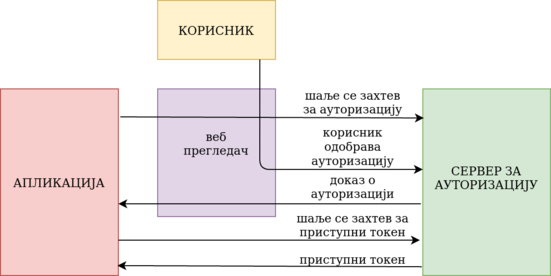
\includegraphics[scale=0.7]{slike/oauth2.png}
  \caption{Процес ауторизације код OAuth2 протокола}
  \label{fig:oauth2}
\end{figure}

Варијанта протокола за апликације од високог поверења подразумева чување клијентског идентификатора и клијентског тајног токена у оквиру саме клијентске апликације. Када се корисник аутентификује, потребно је да приложи корисничко име и лозинку, заједно са клијентским идентификатором и клијентским тајним токеном (клијентски идентификатор и клијентски тајни токен се прилажу имплицитно, од стране апликације). С обзиром да се ради о поузданој клијентској апликацији, кориснички креденцијали неће завршити на неком непознатом серверу. Након успешне аутентификације, сервер враћа приступни токен за приступ заштићеним ресурсима, као и токен за освежавање приступног токена. Од тог тренутка надаље, ова два токена представљају активну сесију, и апликација може да их користи за приступ ресурсима и за одржавање сесије, односно, нема потребе за поновним слањем креденцијала и ризиковањем да их нека трећа страна пресретне у небезбедној мрежи\footnote{Коришћење енкриптованог саобраћаја може помоћи да се креденцијали сакрију од треће стране, али и даље постоје механизми за пресретање оваквог саобраћаја, посебно у необезбеђеним мрежама, или мрежама чији власник није познат.}. Наравно, и даље постоји могућност да се пресретне сам приступни токен, што би нападачу дало приступ корисничком налогу и без поседовања креденцијала. Ово је отворен проблем који и даље нема савршено решење, али опасност од горе наведених ствари се може у потпуности избећи опрезом корисника, тј. избегавањем коришћења необезбеђених и непроверених мрежа, и неприхватањем сертификата који нису потписани од стране неког сертификационог тела од поверења. Такође, апликација би приликом одјављивања корисника, поред брисања приступног токена из локалног складишта уређаја, требало да шаље захтев за поништавање приступног токена. Главна мана ове варијанте OAuth2 протокола је то што се клијентски идентификатор и клијентски тајни токен чувају у самој клијентској апликацији, на клијентском уређају. Уз мање или више муке, реверзним инжењерингом трећа страна може доћи до ових параметара, и направити своју варијанту апликације која може бити небезбедна за употребу. Корисник се може заштитити од овога преузимањем апликација само из проверених извора.

\subsection{Платформа Докер}
Докер је платформа дизајнирана тако да олакша процес креирања, упошљавања и покретања апликација употребом софтверских контејнера. Контејнери омогућавају програмерима да упакују апликацију, библиотеке и све остале зависности заједно у форми пакета. На овај начин се онемогућавају потенцијални проблеми да софтвер на једној машини ради, а на другој не, или да само делимично ради. У секцији \ref{hostovanjeservisa} је речено да су контејнери доста слични виртуелним машинама, али да имају нешто слабији степен виртуелизације, што им омогућава да буду ефикаснији. Контејнери су изоловани једни од других, и могу да комуницирају једни са другима кроз добро дефинисане канале комуникације.

Докер се састоји од клијентске и серверске апликације. Сва интеракција, укључујући покретање и заустављање контејнера, се обавља посредством клијентске апликације која комуницира са сервером користећи Докер REST интерфејс. Основни концепти које Докер користи су слика (енг.~\textit{Docker image}), контејнер и сервис. Једино Докер сервер може директно да манипулише сликама, контејнерима и сервисима.

Слика представља шаблон, односно упутство како се креира контејнер. Паковање апликације и њених зависности у пакет подразумева изградњу слике; процес изградње описује се такозваним Докер датотекама (енг.~\textit{Dockerfile}), где се наводе кораци од којих се изградња састоји. Сама синтакса језика којим се описују ови кораци је слична синтакси Unix љуске (енг.~\textit{Unix shell}). Структура Докер слика је слојевита. Извршавање једног од корака изградње слике резултује креирањем слоја који садржи измене настале извршавањем тог корака. Извршавање сваког наредног корака изградње се ослања на претходно изграђени слој, и у нови слој се додају само измене настале извршавањем текуће инструкције. Разлог овакве организације је то што изменом једног од корака изградње неке слике није потребно извршити поновну изградњу целе слике, већ само почевши од корака који се изменио. У основи сваке Докер слике се налази базна слика (енг.~\textit{base image}), на коју се додаје низ слојева насталих извршавањем скупа инструкција за изградњу.

Контејнер представља конкретан процес у меморији, и покреће се навођењем конкретне слике која ће представљати шаблон за његово креирање. Покретањем контејнера, на постојеће слојеве слике се додаје нови слој у који је могуће уписивати податке, а који ће контејнер користити током свог извршавања. Овај слој је обично јако танак, зато што контејнери у њега уписују само измене у односу на слојеве испод; биће уписане нове датотеке, информације о обрисаним датотекама, и измене постојећих датотека из нижих слојева.

Докер сервиси омогућавају контејнерима да се скалирају хоризинтално између више Докер сервера, чиме се добија скуп Докер сервера (енг.~\textit{swarm}) који међусобно сарађују употребом Докер интерфејса за програмирање апликација (енг.~\textit{Docker API}). Хоризонтално скалирање контејнера подразумева покретање више инстанци сервиса неке апликације на више машина домаћина. Развијена је и алатка Docker Compose \cite{DockerCompose}, чији је циљ да олакша процес организације и управљања контејнерима развијеног софтверског система.

\section{Архитектура и дизајн апликације}
Развијена апликација се може поделити на две велике целине: серверски део (енг.~\textit{backend}) и клијентску апликацију (енг.~\textit{frontend}). Серверски део апликације је организован у микросервисну архитектуру, где сваки сервис има јасно дефинисану одговорност, и где је највећи део доменске логике садржан. Сваки микросервис представља границу једног моделованог поддомена, односно ограничени контекст поддомена. Имплементиране доменске функционалности на серверској страни се на располагање стављају клијентској апликацији, и то кроз добро дефинисан јавни интерфејс. Јавни интерфејс не мора нужно представљати унију интерфејса свих микросервиса, и то обично и није случај. У пракси се обично издваја једна компонента као улазна тачка у систем, и њеним посредством клијентске апликације комуницирају са остатком система. Архитектура развијене апликације је приказана на слици \ref{fig:my-running-buddy}.

Сви микросервиси су развијени употребом Lumen развојног оквира, и користе JSON серијализацију порука која је доследна у целом систему. За потребе складиштења података користи се систем за управљање базама података MySQL, а подаци су организовани тако да сваки микросервис има своју базу података. Подацима из одређене базе података сме да приступа само сервис коме је база намењена. За међусервисну комуникацију користи се Guzzle \cite{guzzle} библиотека за слање HTTP захтева. У наставку ове секције ће бити приказана мотивација за сваку од развијених компоненти, изазови, и тамо где је потребно - имплементациони детаљи.

\begin{figure}[!ht]
  \centering
  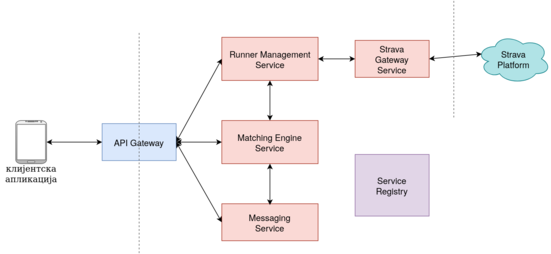
\includegraphics[scale=0.7]{slike/my-running-buddy.png}
  \caption{Архитектура апликације My Running Buddy}
  \label{fig:my-running-buddy}
\end{figure}

\subsection{Cервис \textit{API Gateway}}
Сервис \textit{API Gateway} представља улазну тачку у систем, односно, посредује између клијентске апликације и осталих сервиса. Намена ове компоненте је вишеструка. Једна од битнијих је то да клијентска апликација не мора да зна за локацију и постојање свих сервиса система. Нови сервиси који нуде додатне функционалности могу бити додавани, а апликација не мора да зна за њих. Апликација једино мора да зна за јавни интерфејс, и да систем користи у складу са спецификацијом тог интерфејса.

Овај сервис је скалабилан, по потреби се може покренути више инстанци, и коришћењем балансера оптерећења могуће је контролисати број клијената који се опслужује од стране сваке инстанце. Додатне инстанце поред балансирања оптерећења могу имати и улогу резерви које могу преузети обраду захтева од инстанце која је отказала.

Поред тога што је овај сервис улазна тачка у систем, он има и додатне улоге, односно, није у питању пасивна компонента која само прослеђује захтеве остатку система. Обрадом неких сложенијих захтева, могу се добити одговори који су композитни, тј. одговори који се састоје од више делова, где је сваки део настао као одговор неког сервиса. Сервис \textit{API Gateway} је задужен за оркестрацију ових сложених захтева, као и за агрегацију добијених одговора.

Још једна битна функционалност коју овај сервис обавља је аутентификација корисника, и то коришћењем протокола OAuth2. Ово је једина тачка у којој се врши аутентификација; уколико је корисник аутентификован, захтеви се обрађују, иначе се захтев одбија. Одговорност ауторизације је пребачена на сваки од микросервиса. За протокол OAuth2 је коришћен Laravel пакет за аутентификацију --- Laravel Passport \cite{laravel_passport}, који садржи комплетну имплементацију OAuth2 сервера. Коришћење овог пакета у оквиру Lumen развојног оквира је захтевало додатно прилагођавање \cite{laravel_passport_in_lumen}. Користи се варијанта OAuth2 протокола прилагођена клијентским апликацијама од високог поверења.

\subsubsection{Јавни интерфејс за програмирање апликација}
У табели \ref{tbl:interfejs} је специфициран јавни интерфејс за програмирање апликација који користи клијентска апликација. Јавни интерфејс је имплементиран у оквиру \textit{API Gateway} сервиса.
\begin{small}
\begin{longtable}{ | >{\centering\arraybackslash} m{0.35\linewidth} | m{0.35\linewidth} | m{0.3\linewidth} | }
\hline
\multicolumn{3}{| c |}{\textbf{POST} \textit{/users}}\\*
\nobreakhline
\textbf{опис} & \textbf{захтев} & \textbf{одговор}\\*
\nobreakhline
регистрација новог корисника
&
"email" : обавезно\newline
"password" : обавезно\newline
"name" : обавезно\newline
"surname" : опционо\newline
"aboutme" : опционо\newline
"location" : опционо
&
201 --- успешна обрада\newline
400 --- невалидан захтев\newline
500 --- серверска грешка\\
\hline
\hline
\multicolumn{3}{| c |}{
	\textbf{GET} \textit{/user/\{id\}}
}\\*
\nobreakhline
\textbf{опис} & \textbf{захтев} & \textbf{одговор}\\*
\nobreakhline
дохватање репрезентације корисника
&
&
200 --- успешна обрада\newline
400 --- невалидан захтев\newline
401 --- невалидна сесијa\newline
500 --- серверска грешка
\\
\hline
\hline
\multicolumn{3}{| c |}{
	\textbf{PATCH} \textit{/user/\{id\}} 
}\\*
\nobreakhline
\textbf{опис} & \textbf{захтев} & \textbf{одговор}\\*
\nobreakhline
ажурирање корисничких података
&
"surname" : опционо\newline
"aboutme" : опционо\newline
"location" : опционо
&
200 --- успешна обрада\newline
400 --- невалидан захтев\newline
401 --- невалидна сесијa\newline
500 --- серверска грешка
\\
\hline
\hline
\multicolumn{3}{| c |}{
	\textbf{GET} \textit{/system\_status}
}\\*
\nobreakhline
\textbf{опис} & \textbf{захтев} & \textbf{одговор}\\*
\nobreakhline
дохватање информација о живости интерних сервиса
&
&
200 --- успешна обрада\newline
500 --- серверска грешка
\\
\hline
\hline
\multicolumn{3}{| c |}{
	\textbf{GET} \textit{/user/\{id\}/linked\_services}
}\\*
\nobreakhline
\textbf{опис} & \textbf{захтев} & \textbf{одговор}\\*
\nobreakhline
дохватање информација о спољним налозима корисника
&
&
200 --- успешна обрада\newline
400 --- невалидан захтев\newline
401 --- невалидна сесијa\newline
500 --- серверска грешка
\\
\hline
\hline
\multicolumn{3}{| c |}{
	\textbf{GET} \textit{/user/\{id\}/external\_service\_authorization\_params}
}\\*
\nobreakhline
\textbf{опис} & \textbf{захтев} & \textbf{одговор}\\*
\nobreakhline
дохватање параметара за повезивање са спољним налогом
&
"service\_name" : обавезно
&
200 --- успешна обрада\newline
400 --- невалидан захтев\newline
401 --- невалидна сесијa\newline
500 --- серверска грешка
\\
\hline
\hline
\multicolumn{3}{| c |}{
	\textbf{DELETE} \textit{/user/\{id\}/external\_service/\{service\_name\}}
}\\*
\nobreakhline
\textbf{опис} & \textbf{захтев} & \textbf{одговор}\\*
\nobreakhline
поништавање ауторизације за спољни налог
&
&
200 --- успешна обрада\newline
400 --- невалидан захтев\newline
401 --- невалидна сесијa\newline
500 --- серверска грешка
\\
\hline
\hline
\multicolumn{3}{| c |}{
	\textbf{GET} \textit{/user/\{id\}/stats}
}\\*
\nobreakhline
\textbf{опис} & \textbf{захтев} & \textbf{одговор}\\*
\nobreakhline
дохватање статистике за трчање
&
&
200 --- успешна обрада\newline
400 --- невалидан захтев\newline
401 --- невалидна сесијa\newline
500 --- серверска грешка
\\
\hline
\hline
\multicolumn{3}{| c |}{
	\textbf{GET} \textit{/user/\{id\}/next\_match}
}\\*
\nobreakhline
\textbf{опис} & \textbf{захтев} & \textbf{одговор}\\*
\nobreakhline
враћа следећег потенцијалног партнера за трчање
&
"priority\_field" : опционо
&
200 --- успешна обрада\newline
400 --- невалидан захтев\newline
401 --- невалидна сесијa\newline
404 --- партнер није пронађен\newline
412 --- статистика није доступна\newline
500 --- серверска грешка
\\
\hline
\hline
\multicolumn{3}{| c |}{
	\textbf{POST} \textit{/matcher/match/\{runner\_id\}/\{suggested\_runner\}}
}\\*
\nobreakhline
\textbf{опис} & \textbf{захтев} & \textbf{одговор}\\*
\nobreakhline
прихватање или одбијање потенцијалног партнера за трчање
&
"action" : обавезно
&
200 --- успешна обрада\newline
400 --- невалидан захтев\newline
401 --- невалидна сесијa\newline
500 --- серверска грешка
\\
\hline
\hline
\multicolumn{3}{| c |}{
	\textbf{GET} \textit{/user/\{id\}/matches}
}\\*
\nobreakhline
\textbf{опис} & \textbf{захтев} & \textbf{одговор}\\*
\nobreakhline
дохватање успешних повезивања
&
"num\_of\_results\_per\_page" : опционо\newline
"page" : опционо
&
200 --- успешна обрада\newline
400 --- невалидан захтев\newline
401 --- невалидна сесијa\newline
500 --- серверска грешка
\\
\hline
\hline
\multicolumn{3}{| c |}{
	\textbf{POST} \textit{/user/\{id\}/messages/\{user\_id2\}}
}\\*
\nobreakhline
\textbf{опис} & \textbf{захтев} & \textbf{одговор}\\*
\nobreakhline
слање поруке у оквиру већ постојеће конверзације
&
"message" : обавезно
&
201 --- успешна обрада\newline
400 --- невалидан захтев\newline
401 --- невалидна сесијa\newline
500 --- серверска грешка
\\
\hline
\hline
\multicolumn{3}{| c |}{
	\textbf{GET} \textit{/user/\{id\}/messages}
}\\*
\nobreakhline
\textbf{опис} & \textbf{захтев} & \textbf{одговор}\\*
\nobreakhline
дохватање конверзација за одређеног корисника
&
"page" : опционо\newline
"num\_of\_results\_per\_page" : опционо\newline
"conversations\_newer\_than" : опционо\newline
"conversations\_older\_than" : опционо
&
200 --- успешна обрада\newline
400 --- невалидан захтев\newline
401 --- невалидна сесијa\newline
500 --- серверска грешка
\\
\hline
\hline
\multicolumn{3}{| c |}{
	\textbf{GET} \textit{/user/\{id\}/messages/\{user\_id2\}}
}\\*
\nobreakhline
\textbf{опис} & \textbf{захтев} & \textbf{одговор}\\*
\nobreakhline
дохватање порука из одређене конверзације
&
"page" : опционо\newline
"num\_of\_results\_per\_page" : опционо\newline
"messages\_newer\_than" : опционо\newline
"messages\_older\_than" : опционо
&
200 --- успешна обрада\newline
400 --- невалидан захтев\newline
401 --- невалидна сесијa\newline
500 --- серверска грешка
\\
\hline
\caption{Јавни интерфејс за програмирање апликација}
\label{tbl:interfejs}
\end{longtable}
\end{small}

\subsection{Сервис \textit{Service Registry}}
Сервис \textit{Service Registry}, односно регистар сервиса, је задужен за регистрацију свих инстанци сервиса у оквиру система, и за проверу живости сваког од њих. Уколико један сервис тражи услуге неког другог сервиса, потребно је да зна само назив одредишног сервиса, а разрешавање стварне локације се врши у оквиру регистра сервиса. Једина локација које сви сервиси треба да буду свесни је локација регистра сервиса. Додатно, како би се избегли чести упити ка регистру, сервиси врше кеширање резултата добијених од регистра одређени временски период. Постоји могућност регистровања више инстанци једног истог сервиса, и у том случају регистар враћа све доступне локације, а сервис онда може да одлучи коју локацију да изабере (на основу живости инстанци, или неког другог параметра). Регистрација нових инстанци се може обављати ручно, али је такође могућа и аутоматизација овог процеса, где ће свака нова инстанца да се региструје аутоматски при подизању сервиса.

\subsection{Сервис \textit{Runner Management Service}}
Сервис \textit{Runner Management Service} је одговоран за управљање корисничким подацима, и садржи информације о спољним налозима на које је корисник повезан. Ово је једини сервис који директно сарађује са сервисним пролазима за комуникацију са спољним сервисима (енг.~\textit{external service gateway}), и једини сервис који је свестан њиховог постојања. Сарадња са сервисним пролазима подразумева преузимање репрезентација тркачких активности са спољних сервиса, и њихово прослеђивање ка сервису \textit{Matching Engine Service}.

Доменски модел овог сервиса се налази на слици \ref{fig:runner-management-service-model}. Ентитет \textit{Runner} представља корисника система и садржи основне личне информације корисника. Ентитет \textit{ExternalAccount} описује спољни кориснички налог, и садржи информације заједничке за све спољне сервисе, укључујући токене сесије, датум истека приступног токена и назив сервиса. Ентитет \textit{ExternalService} садржи базичне информације о спољном сервису, у овом случају само прави назив спољног сервиса. Сервис \textit{Runner Management Service} не садржи било какве специфичности везане за одређени спољни сервис, и не зна како да комуницира са спољним сервисима; за тај посао су задужени сервисни пролази, а \textit{Runner Management Service} користи само интерфејс који је заједнички за све сервисне пролазе.

\begin{figure}[!ht]
  \centering
  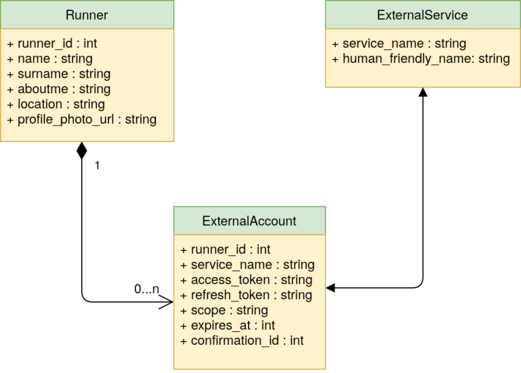
\includegraphics[scale=0.7]{slike/runner-management-service-model.png}
  \caption{Доменски модел сервиса \textit{Runner Management Service}}
  \label{fig:runner-management-service-model}
\end{figure}

\subsection{Сервис \textit{Strava Gateway Service}}
Сервис \textit{Strava Gateway Service} је сервисни пролаз одговоран за комуникацију са спољним сервисом \textit{Strava} \cite{stravaapi}. \textit{Strava} je апликација за праћење физичке активности и снимање тренинга, која укључује популарне функционалности друштвених мрежа, попут коментарисања и прегледа профила других корисника. Сервисни пролази су задужени за све специфичности комуникације са спољним сервисом, и трансформацију формата одговора специфичног спољног сервиса у формат одговора који ће разумети сервис \textit{Matching Engine Service}. Овај сервис је тренутно једини сервисни пролаз у серверском делу апликације, али архитектура апликације омогућава једноставно додавање подршке за нове спољне сервисе; потребно је имплементирати само нови сервисни пролаз за платформу за коју се додаје подршка.

\subsection{Сервис \textit{Matching Engine Service}}
Сервис \textit{Matching Engine Service} садржи логику главног поддомена и представља најбитнији сервис целе апликације. Главне улоге овог сервиса су израчунавање различитих статистика везаних за трчање на основу података из спољних сервиса, и проналажење потенцијалних партнера за трчање. У наставку секције биће описан алгоритам за упаривање тркача.

Алгоритам упаривања је заснован на тркачким статистикама и локацији последње активности. Улазни параметар овог алгоритма је тркач за којег се проналази потенцијални партнер, тј. улазни параметри су статистике овог тркача и локација последње активности.

За разумевање алгоритма, прво је потребно дефинисати појам коефицијента поклапања два тркача. Коефицијент поклапања два тркача се рачуна као збир коефицијената поклапања одговарајућих вредности статистика које алгоритам користи. Статистике које алгоритам користи су приказане у табели \ref{tbl:statistike}.
\begin{table}[h!]
\caption{Статистике које користи алгоритам упаривања}
\label{tbl:statistike}
\centering
\begin{tabular}{ | c | p{0.75\linewidth} | }
\hline
\textbf{ознака} & \multicolumn{1}{| p{0.75\linewidth} |}{\centering \textbf{опис статистике}}\\
\hline
 $s_1$ & укупан број претрчаних километара на недељном нивоу\\
\hline
 $s_2$ & просечно укупно време у покрету на недељном нивоу\\
\hline
 $s_3$ & просечна најдужа дистанца на недељном нивоу\\
\hline
 $s_4$ & просечна брзина\\
\hline
 $s_5$ & просечно време почетка тренинга (рачуна се медијана уместо аритметичке средине)\\
\hline
 $s_6$ & просечан укупан успон на недељном нивоу\\
\hline
\end{tabular}
\end{table}

Функција која је одабрана за рачунање поклапања вредности статистике је $1 - |\widehat{s}_{i,p} - \widehat{s}_{i,q}|$, где су $\widehat{s}_{i,p}$ и $\widehat{s}_{i,q}$ нормализоване вредности неке конкретне статистике $s_i$ за тркаче $p$ и $q$. Разлог за одабир ове функције је то што максимум постиже када су вредности статистике једнаке, а како се разлика између ових вредности повећава, коефицијент поклапања постаје све мањи. На пример, узмимо два тркача и статистику која рачуна просечну брзину. Нека је нормализована вредност ове статистике код првог тркача једнака $0.2$, а код другог тркача $0.9$. Коефицијент поклапања вредности ове статистике износи $1 - |\widehat{s}_{4,1} - \widehat{s}_{4,2}| = 1 - |0.2 - 0.9| = 0.3$. Уколико за нормализовану вредност просечне брзине другог тркача узмемо вредност која је ближа нормализованој вредности првог тркача, нпр. $0.25$, коефицијент поклапања постаје већи --- $1 - |0.2 - 0.25| = 0.95$.

Вредности статистика се нормализују како би свака од статистика имала једнак утицај на коначни коефицијент. Формула за рачунање коефицијента поклапања тркача $p$ и $q$ је: \[ \sum_{i=1}^{numofstats} (1 - |\widehat{s}_{i,p} - \widehat{s}_{i,q}|) \] где је променљива $numofstats$ укупан број статистика које утичу на поклапање. Вредност статистике $s_i$ се нормализујe користећи формулу \[\frac{s_i - \underline{s_i}}{\overline{s_i} - \underline{s_i}}, \underline{s_i} < \overline{s_i}\] где $\underline{s_i}$ и $\overline{s_i}$ представљају опсег придружен статистици $s_i$. Аутор рада је опсеге придружене статистикама изабрао сопственом проценом, и то тако да опсези обухватају већину рекреативних и професионалних тркача. Оваквом нормализацијом се углавном добијају вредности у опсегу $[0, 1]$, али је могуће одступање изван ових граница у ванредним случајевима. Ванредни случајеви подразумевају вредности статистика које одступају од дефинисаних опсега. На пример, за очекиване граничне вредности статистике просечног укупног успона на недељном нивоу су произвољно узете вредности од 0 и 10 километара. Скоро сви тркачи упадају у овај опсег, али ће екстремни случајеви увек постојати. Одступање вредности статистике од дефинисаних оквира не утиче на тачност алгоритма.

Алгоритам функционише тако што прво изабере групу од највише $n$ тркача у радијусу од $d$ километара, а након тога врши рангирање на основу коефицијента поклапања потенцијалних тркачких партнера са улазним тркачем. Након рангирања се узима $m$ резултата са најбољим коефицијентима, где је $m \le n$. Први од њих се враћа као резултат упаривања, а преосталих $m-1$ резултата ће се враћати кроз одговоре наредних захтева, како сваки захтев за проналажење новог партнера не би покретао целокупан алгоритам испочетка.

Додатни опциони параметар овог алгоритма је назив статистике која ће највише утицати на коначни коефицијент поклапања. Ова функционалност је корисна у случају да корисник жели да стави нагласак на одређену карактеристику потенцијалног партнера за трчање, нпр. жели партнера за трчање који му је најсличнији, али жели да се посебан нагласак стави на просечан тотални успон који тркач постиже током једне недеље, уколико је жељени профил партнера тркач који се бави брдско-планинским трчањем. Овај додатни параметар утиче на коначни коефицијент поклапања тако што поклапање жељене статистике скалира за фактор $c$. Вредности $m, n, c$ и $d$ су подесиве на нивоу целог сервиса.

За рачунање одстојања између две локације користи се еквиректангуларна апроксимација \cite{distance_approximation} \[R \cdot \sqrt[2]{(lng_q - lng_p)^2 \cdot cos^2(\frac{lat_p + lat_q}{2}) + (lat_q - lat_p)^2}\] која за велика растојања апроксимацију врши лошије у односу на друге апроксимације. $R$ представља средњи полупречник планете Земље, а $(lat_p, lng_p)$ и $(lat_q, lng_q)$ су координате тачака географског координатног система за тркаче $p$ и $q$ између којих се рачуна растојање. Емпиријском методом је показано да је грешка апроксимације занемарљива за растојања до 50 километара (0.4\% у најгорем случају) \cite{geographic_distance_article}. Овај резултат је више него довољан за потребе апликације која се развија, с обзиром да тачно растојање није неопходно. Разлог за одабир овог начина апроксимације растојања је то што се формула за прорачун састоји од мање рачунски захтевних операција попут тригонометријских функција и квадратног корена. Конкретно, формула еквиректангуларне апроксимације се састоји од само једне косинусне, и једне функције квадратног корена, за разлику од прецизнијих апроксимација попут Haversine формуле \cite{distance_approximation} која је рачунски доста захтевнија.

У наставку је представљен псеудокôд који приказује гореописани процес проналажења потенцијалног партнера за конкретног корисника:
\begin{english}
\lstset{
  language=Python,
  basicstyle=\ttfamily,
  keywordstyle=\color{blue}
}
\begin{lstlisting}
def PronadjiPartnera(idTrkaca):
    postojeciRezultati = PostojeciRezultati(idTrkaca)

    if postojeciRezultati != None:
        return postojeciRezultati[0]

    trkaciURadijusu = NTrkacaURadijusu(userId, N, RADIJUS)
    if trkaciURadijusu == None:
        return None

    listaTrkaca = []
    for trkac in trkaciURadijusu:
        koef = KoeficijentPoklapanja(idTrkaca, trkac.id)
        listaTrkaca.push_back((trkac.id, koef))

    SortirajOpadajucePoKoeficijentuPoklapanja(listaTrkaca)

    prvihMTrkaca = VratiPrvihM(listaTrkaca, M)
    
    SacuvajPostojeceRezultate(prvihMTrkaca)

    return prvihMTrkaca[0]
\end{lstlisting}
\end{english}
Променљиве $N, M$ и $RADIJUS$ одговарају вредностима $n, m$ и $d$ из горенаведeног описа алгоритма. Функције \textit{NTrkacaURadijusu} и \textit{KoeficijentPoklapanja} су такође описане у тексту у оквиру ове секције. Функција \textit{PostojeciRezultati} враћа резултате претходног израчунавања, односно претходног покретања овог алгоритма, уколико су они доступни. Функција \textit{SacuvajPostojeceRezultate} чува резултате текућег извршавања алгоритма. Комплетна имплементација овог процеса се може пронаћи у оквиру имплементације сервиса \textit{Matching Engine Service}, изворна датотека \textit{app/Http/Controllers/MatcherController.php}, метода \textit{find\_partner}.

На слици \ref{fig:spoljni_servis_tok_podataka} је приказан ток података од спољних сервиса до сервиса \textit{Matching Engine Service} где се складиште тркачке активности и рачуна тркачка статистика. Извршавање овог процеса се заказује у оквиру сервиса \textit{Runner Management Service}, аутоматски, са фреквенцијом од 15 минута. У сваком циклусу извршавања, за сваки од спољних налога се проверава време последње синхронизације, и уколико је то време веће од једног дана, захтевају се активности од одговарајућег сервисног пролаза, и то активности новије од времена последње синхронизације. Уколико се спољни налог синхронизује први пут, захтевају се све активности у протекле четири недеље. Добијене активности се прослеђују на сервис \textit{Matching Engine Service}, где се новодобијене активности складиште, активности старије од четири недеље се уклањају, и рачунају се горепоменуте статистике.

\begin{figure}[!ht]
  \centering
  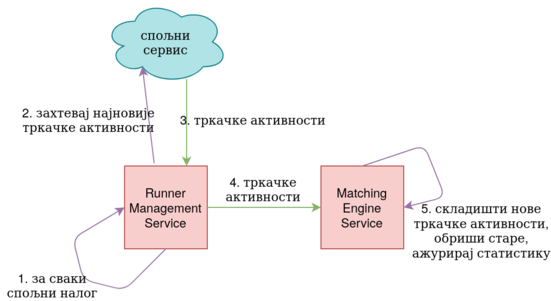
\includegraphics[scale=0.7]{slike/spoljni-servis-tok-podataka.png}
  \caption{Ток података од спољних сервиса до сервиса \textit{Matcing Engine Service}}
  \label{fig:spoljni_servis_tok_podataka}
\end{figure}

\subsection{Сервис \textit{Messaging Service}}
Намена сервиса \textit{Messaging Service} је да омогући међусобну комуникацију већ повезаних тркача. Овај сервис нуди основне функционалности прављења конверзација и слања порука у оквиру конверзација, с тим да прављење конверзација није доступно преко јавног интерфејса, већ се та операција обавља након успешног повезивања два тркача. С обзиром да се ради о сервису чији домен припада генеричкој категорији, постоји велики број готових софтверских решења која би могла да замене ову тривијалну имплементацију.

\subsection{Клијентска апликација}
Поред серверског дела, развијена је и клијентска апликација која користи имплементиране функционалности на серверу. За развој клијентске апликације коришћени су Android комплет за развој софтвера и програмски језик Јава. За мрежну комуникацију са сервером је искоришћена библиотека Volley \cite{volley} која представља имплементацију клијента за HTTP протокол. Како би се поједноставила употреба ове библиотеке за развијени јавни интерфејс, дизајнирана је библиотека APIWrapper, омотач интерфејса који прикрива делове кода специфичне за коришћење мрежне библиотеке и паковање података захтева. Развијен је и још један додатни слој, APIObjectLoader, чија је улога да на једноставан начин учита репрезентацију удаљеног објекта са сервера, заједно са подршком за кеширање објеката и освежавањем приступних токена. На овај начин се раздваја зависност главне логике апликације од мрежне логике и кеширања.

Полазна тачка клијентске апликације је Android активност (енг.~\textit{Android activity}) која проверава да ли је већ ускладиштена сесија корисника. Уколико сесија није ускладиштена, односно ако корисник није пријављен, врши се редирекција на активност за пријављивање. Активност за пријављивање корисника садржи улазна поља за креденцијале корисника, као и везу за редирекцију на активност за регистрацију нових корисника. Изглед активности за пријављивање и регистрацију је приказан на слици \ref{fig:registracija_logovanje}.

\begin{figure}[!ht]
  \centering
  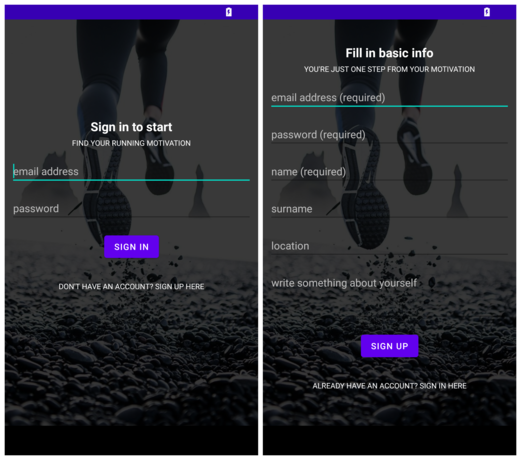
\includegraphics[scale=0.7]{slike/registracija-logovanje.png}
  \caption{Активности за пријављивање и регистрацију}
  \label{fig:registracija_logovanje}
\end{figure}

Уколико је корисник већ пријављен, врши се редирекција на активност за приказ профила пријављеног корисника. Активност за приказ профила приказује основне информације о кориснику, попут имена, профилне слике, личног описа и тркачке статистике. Навигација кроз садржај апликације се врши додиром "хамбургер" дугмета у левом горњем углу, или превлачењем прста са левог на десни крај дисплеја уређаја, након чега се отвара мени за навигацију. Активност корисничког профила и изглед менија за навигацију се налазе на слици \ref{fig:profil_meni}.

\begin{figure}[!ht]
  \centering
  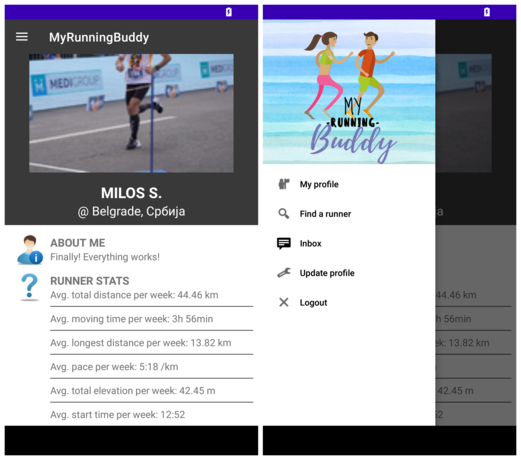
\includegraphics[scale=0.7]{slike/profil-meni.png}
  \caption{Активност корисничког профила и навигација}
  \label{fig:profil_meni}
\end{figure}

Поред представљених активности, апликација поседује активност за ажурирање корисничких података и повезивање са спољним сервисима, активност за проналажење партнера за трчање и активност за комуникацију упарених тркача. Активност за проналажење партнера за трчање представља главну активност у апликацији, и њен изглед је готово идентичан изгледу активности за преглед профила, уз додатак дугмића за прихватање или одбијање предложеног партнера. Након успешног упаривања са неким тркачем, корисник се редиректује на активност за комуникацију, која ће између осталог садржати и тркача са којим је управо упарен. На слици \ref{fig:pretraga_konverzacija} је приказан изглед активности за проналажење партнера и активности за преглед конверзација. Активности везане за комуникацију корисницима дају могућност бољег упознавања, размену контакт информација и заједничко планирање тренинга.

\begin{figure}[!ht]
  \centering
  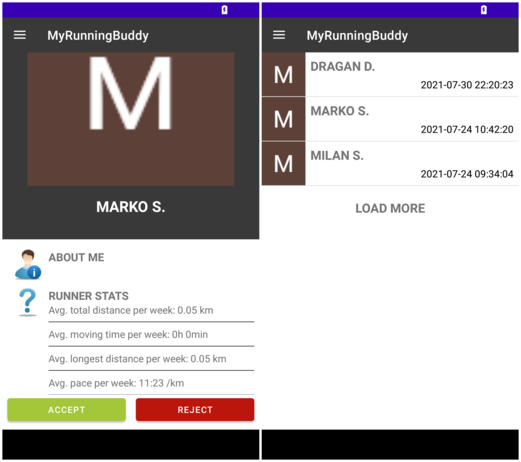
\includegraphics[scale=0.7]{slike/pretraga-konverzacija.png}
  \caption{Активности за проналажење партнера и преглед конверзација}
  \label{fig:pretraga_konverzacija}
\end{figure}

Повезивање корисничког налога са спољним налогом неког сервиса се може вршити из активности за ажурирање профила, додиром дугмета за повезивање са одговарајућим спољним налогом у оквиру секције за спољне налоге. Додиром дугмета за повезивање се отвара веб прегледач са веб локацијом која садржи форму за потврду или одбијање ауторизације. Потврђивањем ауторизације, корисник се обавештава да је повезивање успешно. За највише 15 минута од тренутка повезивања ће бити покренуто аутоматско синхронизовање са спољним сервисом и рачунање тркачке статистике, након чега корисник може да почне са проналажењем партнера за трчање. На слици \ref{fig:azuriranje_autorizacija} је приказана активност за ажурирање корисничког профила и активност веб прегледача која приказује садржај форме за ауторизацију са спољним налогом.

\begin{figure}[!ht]
  \centering
  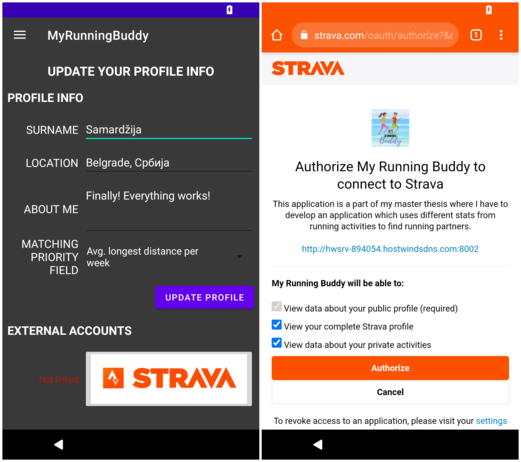
\includegraphics[scale=0.7]{slike/azuriranje-autorizacija.png}
  \caption{Активност за ажурирање корисничког профила и активност веб прегледача са ауторизационом формом}
  \label{fig:azuriranje_autorizacija}
\end{figure}

\section{Тестирање апликације и тестно окружење}
Развојни оквир Lumen нуди једноставан и стандардан начин за писање јединичних и сервисних тестова користећи PHPUnit развојни оквир за тестирање \cite{phpunit}. Lumen садржи компоненте које омогућавају изоловање функција и сервиса који се тестирају од остатка апликације, и то тако што пружа механизме лажирања приступа бази података и мрежној комуникацији. Користећи ове механизме, пре покретања тестова је могуће поставити жељени контекст у којем ће се они извршавати, што омогућава јасно дефинисање жељеног тестног сценарија.

Имплементација серверског дела апликације садржи скуп јединичних и сервисних тестова који покривају најкритичније тачке. Тестови се покрећу позиционирањем на директоријум сервиса чији се тестови покрећу, и извршавањем команде \textit{./vendor/bin/phpunit}. Резултат извршавања ове команде садржи информацију о количини радне меморије која се користила током извршавања тестова, времену извршавања тестова и успешности сваког од тестова. Уколико постоји тест који не пролази, детаљно се исписују информације о позицији и типу грешке, као и о добијеним и очекиваним вредностима.

Сваки сервис додатно садржи Докер датотеке са упутствима за изградњу Докер слика. У кореном директоријуму пројекта серверске апликације се налази датотека \textit{docker-compose.yml} која садржи дефиниције сервиса, приватне рачунарске мреже у оквиру које ће се сервиси извршавати, и портова који ће бити видљиви у склопу оперативног система домаћина (енг.~\textit{host}). Ова датотека се може учитати алатком Docker Compose, која се може искористити за изградњу слика свих сервиса одједном. Изградња слика се врши позиционирањем на директоријум где је лоцирана \textit{docker-compose.yml} датотека, и позивањем команде \textit{docker-compose build -{}-force-rm}. Додатни параметар \textit{-{}-force-rm} ће изазвати брисање свих привремених слика које су настале у процесу изградње сервиса. Ово је посебно корисна опција уколико ће се изградња вршити често, нпр. у оквиру непрекидне интеграције софтвера, јер привремене слике врло брзо могу попунити простор на диску. Такође, могуће је покренути све сервисе позивањем једне команде --- \textit{docker-compose up}. Сваки од дефинисаних сервиса ће бити покренут изоловано, у оквиру свог контејнера. Сервиси у оквиру различитих контејнера ће моћи да комуницирају једни са другима, јер су дефинисани у оквиру исте мреже, а спољном свету ће бити изложени само одабрани сервиси. Контејнери могу бити заустављени покретањем команде \textit{docker-compose stop}, и у овом сценарију контејнери чувају своје стање. Уколико има потребе за заустављањем сервиса и брисањем креираних контејнера и мрежа, може се покренути команда \textit{docker-compose down}.

Све ово омогућава подизање читавог свежег система у року од неколико секунди, што је изузетно корисно за аутоматизовано и мануелно тестирање с краја на крај. Докер се такође може користити и у продукционом окружењу, али слике креиране у оквиру овог пројекта су из више разлога погодне само за тестирање и локалну употребу. Употреба овако дефинисаних слика у продукционом окружењу може представљати велики безбедносни ризик. Креирано тестно Докер окружење користи веб сервер који је уграђен у PHP интерпретер, и који је ограничен у погледу перформанси и подешавања. Ово између осталог подразумева и коришћење неенркиптованог саобраћаја, што није прихватљиво за продукционо окружење. Поред тога, база података се покреће у оквиру истог контејнера где и одговарајући сервис, што није решење које се користи у пракси.

Тестирање креираног система с краја на крај је извршено мануелно, у оквиру тестног окружења, и то коришћењем клијентске апликације са најважнијим случајевима употребе који ће бити описани у наставку секције.

\subsection{Регистрација и пријављивање корисника}
\begin{description}
    \item \textbf{актери} --- корисник
    \item \textbf{предуслови} --- не постоји сачувана активна сесија на уређају
    \item \textbf{постуслови} ---  кориснички налог је креиран, корисник је пријављен
    \item (1) Корисник покреће апликацију и преусмерава се на активност за пријављивање
    \item (2) Корисник додирује тектстуалну ознаку за креирање новог налога и преусмерава се на активност за регистрацију
    \item (3) Корисник попуњава личне податке
    \item (4) Корисник додирује дугме за регистрацију
    \begin{description}
        \item (4.1) Корисник је успешно попунио податке, кориснички налог је креиран и корисник се преусмерава на активност за пријављивање и случај употребе се наставља од корака 5
        \item (4.2) Корисник није успешно попунио податке и случај употребе се наставља од корака 3
    \end{description}
    \item (5) Корисник попуњава креденцијале за пријављивање и додирује дугме за пријављивање
    \begin{description}
        \item (5.1) Корисник је унео валидне креденцијале, успешно је пријављен, преусмерава се на активност за приказ профила и случај употребе се завршава
        \item (5.2) Корисник није унео валидне креденцијале и случај употребе се наставља од корака 5
    \end{description}
    \item \textbf{cпецијални ток} --- 4, 5) неки сервиси неопходни за обављање операције нису активни или имају неки проблем, корисник се обавештава о грешци
    \item \textbf{cпецијални ток} --- 1 - 5) корисник затвара апликацију и случај употребе се завршава 
\end{description}

\subsection{Покушај пријављивања истог корисника истовремено са више уређаја}
\begin{description}
    \item \textbf{актери} --- корисник
    \item \textbf{предуслови} --- корисник је пријављен преко првог уређаја, не постоји сачувана активна сесија на другом уређају
    \item \textbf{постуслови} --- корисник је пријављен преко другог уређаја, сесија са првог уређаја више није активна
    \item (1) Корисник покреће апликацију на другом уређају и преусмерава се на активност за пријављивање
    \item (2) Корисник попуњава креденцијале за пријављивање и додирује дугме за пријављивање
    \begin{description}
        \item (2.1) Корисник је унео валидне креденцијале, успешно је пријављен, сесија са првог уређаја је поништена, корисник се преусмерава на активност за приказ профила и случај употребе се завршава
        \item (2.2) Корисник није унео валидне креденцијале и случај употребе се наставља од корака 2
    \end{description}
    \item \textbf{cпецијални ток} --- 1 - 2) неки сервиси неопходни за обављање операције нису активни или имају неки проблем, корисник се обавештава о грешци
    \item \textbf{cпецијални ток} --- 2) корисник затвара апликацију и случај употребе се завршава 
\end{description}

\subsection{Повезивање са спољним налозима, аутоматска синхронизација података и рачунање тркачке статистике}
\begin{description}
    \item \textbf{актери} --- корисник
    \item \textbf{предуслови} --- корисник је пријављен и налази се на активности за преглед профила, спољни налог сервиса \textit{Strava} није повезан
    \item \textbf{постуслови} --- корисник је успешно повезао спољни налог, тркачке активности ће бити преузете за највише 15 минута и статистика ће бити израчуната
    \item (1) Корисник отвара навигацију, бира опцију за ажурирање профила и преусмерава се на активност за ажурирање профила
    \item (2) Корисник у секцији "спољни налози" додирује дугме за повезивање са спољним сервисом \textit{Strava}, отвара се веб прегледач са веб локацијом за ауторизацију са сервисом \textit{Strava}
    \begin{description}
        \item (2.1) Корисник је ауторизовао приступ спољном сервису са потребним правима приступа, затвара веб прегледач, преусмерава се на активност за ажурирање података где се види информација да је спољни налог успешно повезан и случај употребе се завршава
        \item (2.2) Корисник није ауторизовао приступ спољном сервису, или ауторизација не садржи неопходна права приступа, преусмерава се на активност за ажурирање података и случај употребе се наставља од корака 2
    \end{description}
    \item \textbf{cпецијални ток} --- 1 - 2) неки сервиси неопходни за обављање операције нису активни или имају неки проблем, корисник се обавештава о грешци
    \item \textbf{cпецијални ток} --- 1 - 2) корисник затвара апликацију и случај употребе се завршава
    \item \textbf{cпецијални ток} --- 1 - 2) сесија је постала невалидна, корисник се преусмерава на активност за пријављивање и случај употребе се завршава
\end{description}

\subsection{Укидање приступа спољним налозима}
\begin{description}
    \item \textbf{актери} --- корисник
    \item \textbf{предуслови} --- корисник је пријављен и налази се на активности за преглед профила, спољни налог сервиса \textit{Strava} је повезан
    \item \textbf{постуслови} --- приступ спољном сервису је укинут
    \item (1) Корисник отвара навигацију, бира опцију за ажурирање профила и преусмерава се на активност за ажурирање профила
    \item (2) Корисник у секцији "спољни налози" додирује дугме за укидање приступа спољном налогу сервиса \textit{Strava}, укида се приступ спољном налогу и случај употребе се завршава
    \item \textbf{cпецијални ток} --- 1 - 2) неки сервиси неопходни за обављање операције нису активни или имају неки проблем, корисник се обавештава о грешци
    \item \textbf{cпецијални ток} --- 1 - 2) корисник затвара апликацију и случај употребе се завршава
    \item \textbf{cпецијални ток} --- 1 - 2) сесија је постала невалидна, корисник се преусмерава на активност за пријављивање и случај употребе се завршава
\end{description}

\subsection{Aжурирање корисничких података}
\begin{description}
    \item \textbf{актери} --- корисник
    \item \textbf{предуслови} --- корисник је пријављен и налази се на активности за преглед профила
    \item \textbf{постуслови} --- кориснички подаци су ажурирани
    \item (1) Корисник отвара навигацију, бира опцију за ажурирање профила и преусмерава се на активност за ажурирање профила
    \item (2) Корисник мења жељене податке
    \item (3) Корисник потврђује измене додиривањем дугмета за чување измена
    \begin{description}
        \item (3.1) Измењени подаци су коректни, измена је успешна и случај употребе се завршава
        \item (3.1) Измењени подаци нису коректни, измена није успешна и случај употребе се наставља од корака 2
    \end{description}
    \item \textbf{cпецијални ток} --- 1, 3) неки сервиси неопходни за обављање операције нису активни или имају неки проблем, корисник се обавештава о грешци
    \item \textbf{cпецијални ток} --- 1 - 3) корисник затвара апликацију и случај употребе се завршава
    \item \textbf{cпецијални ток} --- 1, 3) сесија је постала невалидна, корисник се преусмерава на активност за пријављивање и случај употребе се завршава
\end{description}

\subsection{Проналажење потенцијалних партнера за трчање}
\begin{description}
    \item \textbf{актери} --- корисник
    \item \textbf{предуслови} --- корисник је пријављен и налази се на активности за преглед профила
    \item \textbf{постуслови} --- десило се упаривање са другим корисником / није се десило упаривање са другим корисником
    \item (1) Корисник отвара навигацију, бира опцију за проналажење партнера и преусмерава се на одговарајућу активност
    \item (2) Учитава се следећи препоручени тркач
    \begin{description}
        \item (2.1) Пронађен је потенцијални партнер за трчање и случај употребе се наставља од корака 3
        \item (2.2) Корисник није повезан са спољним сервисом, нема тркачку статистику или у том тренутку нема препоручених тркача, и случај употребе се завршава 
    \end{description}
    \item (3) Корисник прегледа профил другог корисника
    \item (4) Корисник врши жељену акцију
    \begin{description}
        \item (4.1) Koрисник прихвата предложеног тркача
        \begin{description}
            \item (4.1.1) Предложени тркач је претходно прихватио упаривање са текућим тркачем, упаривање је комплетирано, текући корисник се преусмерава на активност са конверзацијама где ће видети информацију о новом упаривању и случај употребе се завршава
            \item (4.1.2) Иначе, случај употребе се наставља од корака 2
        \end{description}
        \item (4.2) Корисник не прихвата предложеног тркача и случај употребе се наставља од корака 2
    \end{description}
    \item \textbf{cпецијални ток} --- 1, 2, 4) неки сервиси неопходни за обављање операције нису активни или имају неки проблем, корисник се обавештава о грешци
    \item \textbf{cпецијални ток} --- 1 - 4) корисник затвара апликацију и случај употребе се завршава
    \item \textbf{cпецијални ток} --- 1, 2, 4) сесија је постала невалидна, корисник се преусмерава на активност за пријављивање и случај употребе се завршава
\end{description}

\subsection{Размена порука између повезаних корисника}
\begin{description}
    \item \textbf{актери} --- први корисник, други корисник
    \item \textbf{предуслови} --- први корисник је пријављен и налази се на активности за преглед профила, постоји успешно упаривање првог и другог корисника
    \item \textbf{постуслови} --- први корисник је успешно послао бар једну поруку другом кориснику
    \item (1) Први корисник отвара навигацију, бира опцију за преглед конверзација и преусмерава се на активност за преглед конверзација
    \item (2) Први корисник додирује конверзацију која се односи на другог корисника и преусмерава се на активност за преглед одређене конверзације
    \item (3) Први корисник чита поруке у оквиру конверзације
    \item (4) Први корисник шаље жељену поруку другом кориснику и случај употребе се наставља од корака 3
    \item \textbf{cпецијални ток} --- 1, 2, 4) неки сервиси неопходни за обављање операције нису активни или имају неки проблем, корисник се обавештава о грешци
    \item \textbf{cпецијални ток} --- 1 - 4) корисник затвара апликацију и случај употребе се завршава
    \item \textbf{cпецијални ток} --- 1, 2, 4) сесија је постала невалидна, корисник се преусмерава на активност за пријављивање и случај употребе се завршава
\end{description}

\subsection{Одјављивање из текуће сесије}
\begin{description}
    \item \textbf{актери} --- корисник
    \item \textbf{предуслови} --- корисник је пријављен и налази се на активности за преглед профила
    \item \textbf{постуслови} --- корисник је успешно одјављен
    \item (1) Први корисник отвара навигацију, бира опцију за одјављивање, преусмерава се на активност за пријављивање и случај употребе се завршава
    \item \textbf{cпецијални ток} --- 1) неки сервиси неопходни за обављање операције нису активни или имају неки проблем, корисник се обавештава о грешци
    \item \textbf{cпецијални ток} --- 1) корисник затвара апликацију и случај употребе се завршава
\end{description}

\section{Извршавање апликације у продукционом окружењу}
У секцији \ref{hostovanjeservisa} су описани могући начини хостовања сервиса. Коришћење било којег од наведених приступа у продукционом окружењу је валидно. У оквиру ове секције ће бити дат кратак преглед инфраструктурних препорука и препорука за подешавање које би требало испратити током пуштања развијеног система у продукционо окружење. С обзиром да се претходна секција бавила Докером, ова секција ће се надовезати на њу, и приказати подешавање продукционог окружења на примеру Докера. Велики део описаних препорука ће бити примењив и у оквиру других приступа хостовања сервиса.

Прва детаљ на који треба обратити пажњу је база података. Пракса је да се издвоји засебан софтверски контејнер за сваку од база података у систему. У терминима развијеног система, то значи да би сваки микросервис требало да има своју базу података, и свака од база података би требало да буде издвојена у свој контејнер. Разлог за овакав приступ, уместо покретања базе података у оквиру контејнера где се извршава микросервис, је правилна иницијализација и деиницијализација сервиса базе података. За овакве потребе су већ доступне унапред изграђене базне слике за различите системе за управљање базом података, које ће се правилно иницијализовати приликом подизања контејнера, и током гашења контејенера правилно деиницијализовати. У супротном, уколико се овај посао ради мануелно у оквиру прилагођених контејнера, велика је вероватноћа да ће се овај процес извести погрешно, што може довести до оштећења или тоталног губитка података. Поред издвајања базе података у засебан контејнер, препоручује се коришћење дељеног система датотека за локацију где систем за управљање базом података складишти податке. Ово се постиже коришћењем механизма Docker volume \cite{dockervolume} који омогућава монтирање дела система датотека домаћинског оперативног система у оквиру самог контејнера\footnote{Заправо, дељење система датотека није ограничено само на домаћински оперативни систем, већ је могуће монтирати и системе датотека удаљених машина и машина у облаку.}, чиме се избегава складиштење важних података у контејнеру, олакшава се дељење података између више контејнера и процес померања сервиса на друге машине се лакше обавља. У пракси се, заустављањем сервиса, чешће уништавају контејнери уместо да се заустављају и поново користе током поновног покретања сервиса. У таквим случајевима је неопходно коришћење механизма дељеног система датотека.

Друга битна измена коју је потребно направити у продукционом окружењу је омогућавање HTTPS протокола за размену података, односно HTTP протокола са додатним слојем енкрипције података. Коришћење енкрипције између клијентске апликације и улазне тачке система је неопходно, док је енкрипција комуникације између сервиса опциона, и зависи од инфраструктуре у којој се сервиси покрећу. Разлог за коришћење енкрипције је прикривање осетљивих података које размењују клијентска апликација и сервер. Додатна корист од енкрипције је и тежа анализа протокола комуникације, што је посебно корисно код апликација које се ослањају на тајност протокола комуникације; међутим, анализа протокола се може извршити и реверзним инжењерингом клијентске апликације.

Продукциони систем треба да буде подешен тако да су сви сервиси осим улазне тачке недоступни за спољашњи свет\footnote{Тестно окружење је подешено тако да је поред улазне тачке видљив и сервис \textit{Service Registry} зарад веће контроле над процесом регистрације сервиса током писања тестова с краја на крај.}, на шта се развијени сервиси и ослањају. Аутентификација корисника система се врши само на улазу у систем, а након тога се идентификација аутентификованог корисника прослеђује кроз захтеве који залазе дубље у систем. Такође, веб сервер улазне тачке би требало да буде подешен тако да врши лимитирање броја захтева који пристижу у јединици времена, како би се спречило онеспособљавање система слањем масивног броја валидних захтева.

\section{Могућа унапређења апликације}
Развијена апликација садржи све основне функционалности које су јој неопходне да би била употребљива. Међутим, постоји доста простора за унапређење постојећих функционалности, и додавање нових, од којих су најбитније образложене у наставку текста.

\subsection{Коришћење ефикаснијих компоненти за кеширање}
Тренутна имплементација серверског дела апликације као кеш користи релациону базу података, тачније, сваки сервис има једну табелу намењену за чување парова кључ-вредност. Ово решење је прихватљиво, али порастом броја захтева који улазе у систем, компонента која се користи за кеширање мора бити у стању да се скалира. Релационе базе података нуде скалабилност, али су за ове сврхе популарније и ефикасније специјализоване софтверске компоненте за кеширање попут Memcached \cite{memcached} и Redis \cite{redis} система. Једина мана код употребе ових система је то што су нешто тежи за подешавање и компликују упошљавање софтвера.

Развојни оквир Lumen омогућава једноставну замену једног подсистема за кеширање другим, без потребе за мењањем постојећег кода који користи кеширање. Развојни оквир ово постиже тако што програмерима нуди интерфејс за кеширање, а у позадини се адаптерима врши прилагођавање различитим подсистемима.

\subsection{Oграничавање броја захтева}
Oво подразумева ограничавање укупног броја захтева по кориснику који улази у систем у јединици времена, како би се спречило онемогућавање услуге од стране злонамерних корисника. Ово може бити решено на нивоу самог веб сервера који опслужује захтеве, као и у оквиру улазне тачке у систем, тј. у оквиру \textit{API Gateway} сервиса.

Друга ставка која је сличне природе, али чија мотивација није везана за перформансе је ограничавање броја упаривања које корисник може имати у неком временском периоду. Овиме се кориснику онемогућава да брзо исцрпи базу могућих партнера, чиме се умањује шанса да корисник кратко користи апликацију и брзо изгуби интересовање, и охрабрује се коришћење апликације дужи временски период.

\subsection{Детаљнији механизми за надгледање сервиса}
Тренутни механизам за надледање сервиса укључује слање једноставних специјалних захтева сервисима, који као резултат пружају информацију о томе да ли је сервис доступан или не. Пожељно је постојање различитих захтева који различитим путањама пролазе кроз цео систем, и који кроз резултат нуде прецизнију слику о стању система.

\subsection{Уклањање постојећих упаривања из листе партнера за трчање}
Потребно је омогућити корисницима функционалност за прекидање везе и комуникације са упареним тркачима. Ово би корисницима омогућило да зауставе потенцијалне непримерене кориснике. Такође, неопходна је функционалност за пријављивање свих врста неправилности.

\subsection{Потврда е-маил адресе након регистрације корисника}
Како би се избегло масовно креирање лажних налога, потребно је увести верификацију налога путем е-маил адресе. Ово није савршено решење, с обзиром да постоје веб сервиси за брзо креирање привремених адреса, али у великој мери смањује број лажних налога.

\chapter{Закључак}
Овај рад је обрадио основне концепте и принципе микросервисне архитектуре, и приказао њихову примену на примеру развијене апликације. Направљена је и паралела између доменски оријентисаног моделовања и микросервисне архитектуре, што демистификује порекло описаних концепата и показује да је микросервисна архитектура нешто више од саме поделе монолитних апликација. Микросервиси деле систем, али га деле тако што у сам центар поделе стављају домен проблема. Рад такође прави осврт на технологију софтверских контејнера (посебно на Докер), који су готово неизоставни део дистрибуираног софтвера, и даје добру почетну тачку за даље истраживање материје.

Серверски део развијене апликације представља пример поделе већег проблема на мање целине, где је свака од целина конкретна имплементација микросервиса који обавља добро дефинисан посао. На примеру тестног окружења је приказано како сервиси могу бити покренути као део целине, и то употребом софтверских контејнера. Развијена Android апликација приказује како клијентске апликације могу користити креирани дистрибуирани систем.

Приказане су предности микросервисне архитектуре, али и мане које би требало да ставе до знања да се не ради о "швајцарском ножу" у развоју софтвера. Микросервиси у великој мери могу олакшати развој и одржавање софтвера, али га исто тако могу и закомпликовати уколико се оваква архитектура форсира тамо где такво решење није природно. Концепти попут интезивне комуникације са доменским експертима, развијања заједничког језика и прављења аналитичког модела могу бити корисни и примењени и у оквиру других архитектура. Рад је дотакао само кључне делове једне велике области, и даљи радови на тему микросервиса и дистрибуираних система се детаљније могу бавити скалирањем, надгледањем, одржавањем и прављењем компромиса код овако развијених система.

\literatura

\backmatter

\begin{biografija}
\textbf{Милош Самарџија} (\emph{Книн, Хрватска, 2. август 1994.}) је дипломирани информатичар Универзитета у Београду и тренутно ради као софтверски инжењер у компанији Teletrader. Завршио је Електротехничку школу "Никола Тесла", смер Електротехничар рачунара, 2013. године у Београду. Исте године уписао је Математички факултет у Београду, смер Информатика, и дипломирао у јулу 2016. године са просечном оценом 8.76. По завршетку основних академских студија уписао је мастер студије, и у току академске 2017-2018 године положио све испите предвиђене планом и програмом мастер студија, са просечном оценом 9.54. У октобру 2018. године се запослио у компанији Teletrader, у тиму који одржава дистрибуирани систем за обраду, складиштење и даље дистрибуирање података са светских берзи у реалном времену. Тренутно ради у истом тиму и усавршава своје знање у области архитектуре софтвера, сајбер безбедности и рачунарских мрежа.
\end{biografija}

\end{document} 
